\documentclass[10pt,a4paper]{article}
\usepackage[margin=1.8cm,top=2.0cm,bottom=2.0cm]{geometry}
\usepackage[utf8]{inputenc}
\usepackage[T1]{fontenc}
\usepackage{lmodern}
\usepackage{xcolor}
\usepackage{amsmath,amssymb}
\usepackage{graphicx}
\usepackage{booktabs}
\usepackage{tabularx}
\usepackage{subcaption}
\usepackage{enumitem}
\setlist{noitemsep,topsep=3pt,parsep=1pt}
\usepackage{lineno}
\usepackage[numbers,super,sort&compress]{natbib}
\usepackage[colorlinks=true,linkcolor=blue!70!black,citecolor=blue!70!black,urlcolor=blue!70!black]{hyperref}
\usepackage[protrusion=true,expansion=true]{microtype}
\usepackage{float}
\usepackage{url}
\usepackage{caption}

% Improve hyphenation and margin alignment
\emergencystretch=2em

% Figure path
\graphicspath{{figures/}{../docs/assets/}}

\title{\textbf{\Large Cross-Study Meta-Analysis of the Gut-Microbiota-Microglia Axis Uncovers Cell-Intrinsic Interferon Shutoff, Invariant Nutrient-Sensing Adapters, and Multi-Omic Reversibility}}

\author{
  \textbf{Samyak Meshram}$^{1,*}$, \textbf{Dr. Soumya Dhokey}$^{1}$ \\[0.4em]
  \small $^{1}$Independent Researchers, Open-Science Initiative \\
  \small $^*$Correspondence: \texttt{sam.meshram18@gmail.com} \quad $|$ \quad GitHub: \url{https://github.com/samyakmeshram/NeuroGut-MetaSeq}
}

\date{\small \today}

\begin{document}

\maketitle

% Start line numbering after title header for reviewer commentary
\linenumbers

\begin{abstract}
Microglia are the resident immune sentinels and parenchymal phagocytes of the central nervous system (CNS), continuously calibrated by biochemical cues from the indigenous gut microbiota. While individual transcriptomic studies have revealed that gut microbiome depletion compromises microglial ramification and immune alertness, findings across laboratories have suffered from small sample sizes, isolation technology carryover, and disparate experimental models. Here, we present \textbf{NeuroGut-MetaSeq (v1.4.0)}, an integrated multi-cohort and multi-omic meta-analysis framework synthesizing 60 biological transcriptomes across four independent rodent cohorts spanning lifelong germ-free (GF) isolation, acute broad-spectrum antibiotic (ABX) cocktails, and dietary fiber starvation. Using negative binomial generalized linear models, Restricted Maximum Likelihood (REML) variance estimation, and Hartung-Knapp-Sidik-Jonkman (HKSJ) small-sample random-effects pooling across 23,096 common genes, we separate an invariant multi-study core from model-private perturbation shocks. We identify an omnipresent invariant core led by the basolateral polarity adapter \textit{Llgl2} ($k=4, \hat{\theta}_{\text{RE}} = +0.672, \text{HKSJ } 95\% \text{ CI } [0.166, 1.178], I^2 = 0.0\%$) and extracellular chaperone hub \textit{Clu} ($k=3, \hat{\theta}_{\text{RE}} = +0.873, I^2 = 0.0\%$), alongside universal loss of myeloid quiescence via \textit{Slfn2} ($k=4, \hat{\theta}_{\text{RE}} = -0.465, p_{\text{HKSJ}} = 0.0197$) and chromatin corepressor \textit{Sap30} ($I^2 = 0.0\%, p_{\text{HKSJ}} = 0.0409$). Paradoxically, acute antibiotic shock markers \textit{Tsc22d3} (GILZ) and \textit{Ddit4} (REDD1) exhibit extreme between-study heterogeneity ($I^2 > 95\%$), classifying them as transient perturbation effectors rather than core dysbiosis hits. 

Factorial sex-interaction modeling across 51 sex-informative samples reveals that \textbf{99.1\% of the microglial response to microbiome depletion is sex-invariant} ($I^2_{\text{sex}} = 0.0\%$), with master regulators \textit{Irf1} ($p = 0.863$) and \textit{Stat1} ($p = 0.362$) showing identical shutdown across sexes, while uncovering selective male-biased vulnerability in quiescence checkpoint \textit{Slfn2} ($\hat{\theta}_{\text{int}} = +0.338, p = 0.017$) and \textit{Oas1a} ($\hat{\theta}_{\text{int}} = +0.335, p = 0.051$). Whole-transcriptome Gene Set Enrichment Analysis (GSEA) and TRRUST upstream regulon deconvolution establish the collapse of basal tonic interferon surveillance (\texttt{\small Hallmark Interferon Gamma Response} NES = -2.274, FDR < 0.001; \texttt{\small Interferon-Responsive Microglia} NES = -2.133, FDR < 0.001), accompanied by coordinated suppression of cell-cycle programs (\texttt{\small G2M Checkpoint} NES = -2.155, \texttt{\small E2F Targets} NES = -1.779), and pinpointing master transcription factor \textbf{IRF1} as the upstream regulon driver ($Z = -2.453, p = 0.00098, \text{FDR} = 0.0380$). High-resolution single-cell deconvolution (BayesPrism, $\kappa = 1.54 < 30$) establishes that Interferon-Responsive Microglia (IRM) are physically preserved ($17.5\%$ depleted vs $16.8\%$ reference), proving that the collapse is a genuine \textbf{cell-intrinsic per-cell transcriptional shutoff} ($p < 0.001$). 

Tripartite microglial ATAC-seq footprinting (Erny 2021) directly demonstrates that TOBIAS open chromatin footprints at \textit{Irf1} and \textit{Stat1} promoter motifs collapse during depletion and are \textbf{88.9\% restored} upon short-chain fatty acid (SCFA) repletion. In silico NicheNet ligand-receptor prioritization identifies circulating bacterial outer membrane vesicles (TLR4/CD14, $r = 0.658$) and brain microvascular endothelial \textit{Ifnb1} (IFNAR1/2, $r = 0.600$) as primary upstream drivers of basal IRF1 tone. Finally, co-expression analysis reveals coordinate upregulation of \textit{Llgl2} and the large neutral amino acid transporter \textbf{LAT1 (\textit{Slc7a5})} (+0.641 LFC) alongside mTOR suppression (-0.469 LFC), establishing an invariant nutrient-scavenging adaptation. We resolve the in vivo blood-brain barrier (BBB) pharmacokinetic paradox through a Three-Pillar relay framework (border-associated macrophages, ACSS2/acetate central metabolic replenishment, and vagal signaling). Together, these multi-omic findings prove that gut microbiome depletion induces an aberrant hybrid state of blunted antiviral surveillance and metabolic scavenging characterized by \textbf{chromatin-poised transcriptional reversibility} upon microbial metabolite restoration.
\end{abstract}

\vspace{0.8em}
\noindent\textbf{Significance Statement:}\newline
Communication along the gut-brain axis is essential for neurodevelopment and immune homeostasis, yet how distal gut microbes maintain microglial vigilance without provoking neuroinflammation has remained elusive. By synthesizing multi-cohort RNA-seq datasets with REML-HKSJ small-sample statistical adjustments, factorial sex-interaction modeling, and BayesPrism single-cell deconvolution, we resolve long-standing discrepancies in the literature, proving that dramatic single-study hits (\textit{Tsc22d3}, \textit{Ddit4}) were uncoupled antibiotic-shock artifacts while interferon surveillance collapse is a sex-invariant, cell-intrinsic program governed by master regulator IRF1. Anchoring these findings in empirical microglial ATAC-seq footprinting demonstrates that this transcriptomic state is a chromatin-poised program that is candidate-reversible by microbial short-chain fatty acids, establishing coordinated transcriptional and chromatin accessibility remodeling consistent with microbial epigenetic cues for therapeutic metabolite interventions in neuroinflammatory disease.



\vspace{1.5em}
\section{Introduction}
Microglia constitute approximately 10\% of cells within the healthy adult mammalian brain parenchyma, serving as primary immune sentinels, sculptors of synaptic connectivity, and guardians of neurovascular integrity\cite{colonna2017_1,prinz2019_2}. Unlike peripheral bone-marrow-derived macrophages, microglia arise exclusively during early embryogenesis from uncommitted c-Kit$^{+}$ erythromyeloid progenitors in the extra-embryonic yolk sac\cite{ginhoux2010_3}. Following migration into the nascent cephalic mesenchyme prior to blood-brain barrier closure, microglia establish a self-sustaining parenchymal population that endures throughout the organism's lifespan via local, low-rate self-renewal without replenishment from circulating monocytes\cite{hashimoto2013_4,askew2017_5}.

Over the past decade, a growing body of work has revealed that the physiological maturity, morphological ramification, and immune competence of adult microglia are not cell-autonomous, but depend upon continuous, active signaling from the indigenous gastrointestinal microbiota\cite{erny2015_6,cryan2019_7}. In a pioneering study, Erny et al. demonstrated that adult mice reared under germ-free (GF) conditions, or treated transiently with broad-spectrum oral antibiotics (ABX), display microglia with immature, hyper-ramified process arborization, enlarged soma, and blunted immune reactivity to bacterial endotoxin\cite{erny2015_6}. Strikingly, recolonization with complex microbiota or oral supplementation with bacterial fermentation end-products---short-chain fatty acids (SCFAs: acetate, propionate, and butyrate), which serve as key molecular transducers between the gut microbiota and host physiology\cite{koh2016_33,smith2013_34,sadler2020_35,sampson2016_36}---was sufficient to rescue microglial morphological and transcriptomic defects\cite{erny2015_6,erny2021_8}. Subsequently, Mossad et al. (2022) and related work demonstrated that gut microbiota-derived cues drive tonic baseline type I/II interferon signaling in brain microglia, sustaining antiviral alertness\cite{mossad2021_9,mossad2022_10}.

Despite these groundbreaking findings, individual transcriptomic studies exploring the gut-microglia axis have frequently arrived at divergent conclusions regarding which specific gene programs are altered\cite{sharon2016_11,abdelhaq2019_12}. While some single-cohort investigations report widespread repression of homeostatic checkpoints (\textit{Tmem119}, \textit{Cx3cr1}, \textit{P2ry12})\cite{thion2018_13}, others observe significant baseline priming of immediate-early transcription factors (\textit{Fos}, \textit{Jun}, \textit{Egr1}), or unperturbed homeostatic expression profiles\cite{spichak2021_14,honda2016_15}. These discrepancies stem from five fundamental technical and biological vulnerabilities in the existing literature:
\begin{enumerate}
\item \textbf{Sample Size Constraints \& Small-Cohort Statistical Vulnerabilities}: Bulk RNA-sequencing of primary isolated microglia typically yields only $n=3$ to $6$ biological replicates per condition. Classical meta-analysis methods like DerSimonian-Laird (DL) are prone to underestimating between-study variance $\tau^2$ when the number of cohorts is small ($k < 5$), generating anti-conservative confidence intervals and false-positive inflation. Restricted Maximum Likelihood (REML) combined with the Hartung-Knapp-Sidik-Jonkman (HKSJ) adjustment ($t_{k-1}$ critical distribution) is required to ensure robust confidence interval coverage.
\item \textbf{Cell Isolation Protocol Confounding}: Primary isolation requires enzymatic digestion and mechanical dissociation, which can induce artifactual ex vivo stress activation signatures (\textit{Fos}, \textit{Atf3}, \textit{Hspa1a})\cite{van2017_16,marsh2022_17}, or vary between fluorescence-activated cell sorting (FACS), magnetic sorting (MACS), or Percoll gradients\cite{bttcher2019_18}.
\item \textbf{Biological Perturbation Heterogeneity}: Experimental paradigms span lifelong germ-free housing (which alters embryonic neurodevelopment and blood-brain barrier permeability)\cite{braniste2014_19}, acute pharmacological antibiotic cocktails (which cause mucosal shock and mitochondrial toxicities)\cite{kennedy2020_20}, and dietary fiber starvation (which deprives the host of fermentable substrate without eradicating microbial biomass)\cite{matt2023_21}.
\item \textbf{The Sex-Dimorphism Blind Spot}: Microglia exhibit pronounced sexual dimorphism in baseline maturation and immune vigilance\cite{thion2018_13}. Most transcriptomic pipelines treat sex purely as an additive nuisance covariate (\texttt{\small ~ sex + condition}), obscuring sex-by-microbiome interaction effects ($\sim \text{sex} \times \text{condition}$).
\item \textbf{The Bulk RNA-Seq Bottleneck \& Epigenomic Disconnect}: Bulk transcriptomic profiling averages across cell populations, unable to distinguish whether blunted interferon signatures reflect a uniform per-cell transcriptional shutoff or depletion of the rare Interferon-Responsive Microglia (IRM) subpopulation. Furthermore, asserting epigenetic reversibility without direct chromatin accessibility profiling leaves the mechanistic chain of custody incomplete.
\end{enumerate}
To resolve these challenges, we engineered \textbf{NeuroGut-MetaSeq (v1.4.0)}. We synthesized 60 biological transcriptomes across four independent rodent cohorts using negative binomial modeling, REML variance estimation, and Hartung-Knapp-Sidik-Jonkman random-effects adjustments across 23,096 common genes. We established a Two-Tier Subgroup Decomposition separating shared microbial tonic surveillance from model-private perturbation shocks, implemented factorial sex-interaction meta-regression across 51 sex-informative samples, resolved the bulk RNA-seq bottleneck through BayesPrism 5-state deconvolution, provided direct chromatin validation through tripartite microglial ATAC-seq footprinting (Erny 2021), mapped upstream cerebrovascular drivers via NicheNet, and resolved the in vivo blood-brain barrier (BBB) pharmacokinetic paradox.



\vspace{1.5em}
\section{Results}
\subsection{Act 1: Multi-Cohort Harmonization, Experimental Paradigms \& Study Architecture}
To establish a rigorous multi-cohort foundation, we systematically curated public RNA-sequencing accessions from the NCBI Gene Expression Omnibus (GEO) conforming to strict biological criteria: (1) isolated primary murine microglia, (2) high-throughput bulk RNA sequencing with integer read count matrices, and (3) annotated experimental conditions contrasting gut microbiota depletion or metabolite manipulation against colonized controls. 

We curated 60 biological samples across four distinct experimental cohorts (\textbf{Table 1}, \textbf{Supplementary Table S1}):
\begin{itemize}
\item \textbf{GSE107925} ($n=25$): Specific-Pathogen-Free (SPF) colonized vs. lifelong Germ-Free (GF) adult male and female mice; CD11b$^{+}$ CD45$^{\text{low}}$ FACS-sorted microglia\cite{thion2018_13}.
\item \textbf{GSE108045} ($n=12$): Vehicle-treated control vs. broad-spectrum antibiotic cocktail (ABX; ampicillin, vancomycin, neomycin, metronidazole) adult male and female mice; FACS-sorted microglia\cite{thion2018_13}.
\item \textbf{GSE186210} ($n=14$): Standard fiber diet vs. zero-fiber (SCFA-deficient) diet in wild-type adult mice; MACS-isolated microglia\cite{matt2023_21}.
\item \textbf{GSE266602} ($n=9$): Colonized (SPF\_Sham) vs. Germ-Free (GF\_Sham) adult mice; Percoll density gradient isolated microglia\cite{wang2024_22}.
\end{itemize}
To resolve how gut-derived signals reach the CNS, we formulated a three-compartment circuit architecture mapping the communication relay from the gastrointestinal lumen across the blood-brain barrier (BBB) to resting parenchymal microglia (\textbf{Figure 1A}). Sequencing library depth across all 60 biological libraries ranged from 1.2 million to 70.4 million mapped reads (mean 20.8 million) (\textbf{Figure 1B}, \textbf{Supplementary Figure S1A}). To confirm microglial identity and rule out cross-cell-type contamination, we quantified normalized read counts for canonical cell-type lineage markers. In FACS-sorted cohorts (GSE107925 and GSE108045), microglial checkpoint genes (\textit{Cx3cr1}, \textit{P2ry12}, \textit{Tmem119}, \textit{Hexb}, \textit{Csf1r}) accounted for >99.2\% of lineage-defining reads, with negligible signal from astrocytes (\textit{Gfap}, \textit{Aqp4}), oligodendrocytes (\textit{Mbp}, \textit{Olig2}), or neurons (\textit{Rbfox3}, \textit{Snap25}) (\textbf{Figure 1C}, \textbf{Supplementary Figure S1B--C}). In Percoll-isolated GSE266602, low-level astrocytic marker reads were detected (\textit{Aqp4} $\sim 2.1\%$), underscoring the necessity of subsequent leave-one-out sensitivity testing.

To ensure that observed differential expression reflected true in vivo biological phenomena rather than mechanical tissue dissociation artifacts, we evaluated a composite ex vivo enzymatic dissociation stress score comprising immediate-early and heat-shock genes (\textit{Fos}, \textit{Jun}, \textit{Egr1}, \textit{Atf3}, \textit{Hspa1a})\cite{van2017_16,marsh2022_17}. Two-sample Welch's $t$-tests and Mann-Whitney $U$ tests revealed no statistically significant differences in isolation stress scores between control and microbiome-depleted microglia across cohorts ($p = 0.683$ in GSE107925, $p = 0.180$ in GSE108045, $p = 0.755$ in GSE186210, $p = 1.0$ in GSE266602) (\textbf{Supplementary Figure S1D}). Principal Component Analysis (PCA) across all 60 biological libraries projected global transcriptomic variance onto PC1 (20.8\% variance, capturing biological depletion vs. colonized status) and PC2 (9.0\% variance, capturing baseline cohort variance) (\textbf{Figure 1D}). Thus, isolation-induced stress does not confound cross-cohort comparisons, establishing a sound multi-cohort baseline.




\begin{table}[htbp]
\centering
\caption{\textbf{Summary of Curated Microglial RNA-Seq Cohorts in NeuroGut-MetaSeq.}}
\label{tab:cohort_summary}
\resizebox{\textwidth}{!}{%
\begin{tabular}{llllcll}
\toprule
\textbf{Cohort} & \textbf{Reference} & \textbf{Experimental Paradigm} & \textbf{Samples ($n$)} & \textbf{Sex} & \textbf{Cell Isolation} & \textbf{Platform} \\
\midrule
\textbf{GSE107925} & Thion et al., \textit{Cell} 2018 & Lifelong Germ-Free vs. SPF Control & 25 & 13M/12F & FACS CD11b$^{+}$CD45$^{\text{low}}$ & HiSeq 2500 \\
\textbf{GSE108045} & Thion et al., \textit{Cell} 2018 & Broad-Spectrum Antibiotics vs. Control & 12 & 6M/6F & FACS CD11b$^{+}$CD45$^{\text{low}}$ & HiSeq 2500 \\
\textbf{GSE186210} & Matt et al., \textit{J Neurosci} 2023 & Zero-Fiber Diet vs. Standard Fiber & 14 & 7M/7F & MACS CD11b Microbeads & NovaSeq 6000 \\
\textbf{GSE266602} & Wang et al., \textit{Exp Neurol} 2024 & Germ-Free vs. Colonized SPF & 9 & Male Only & Percoll Gradient & NovaSeq 6000 \\
\bottomrule
\end{tabular}%
}
\end{table}
\begin{figure}[htbp]
\centering
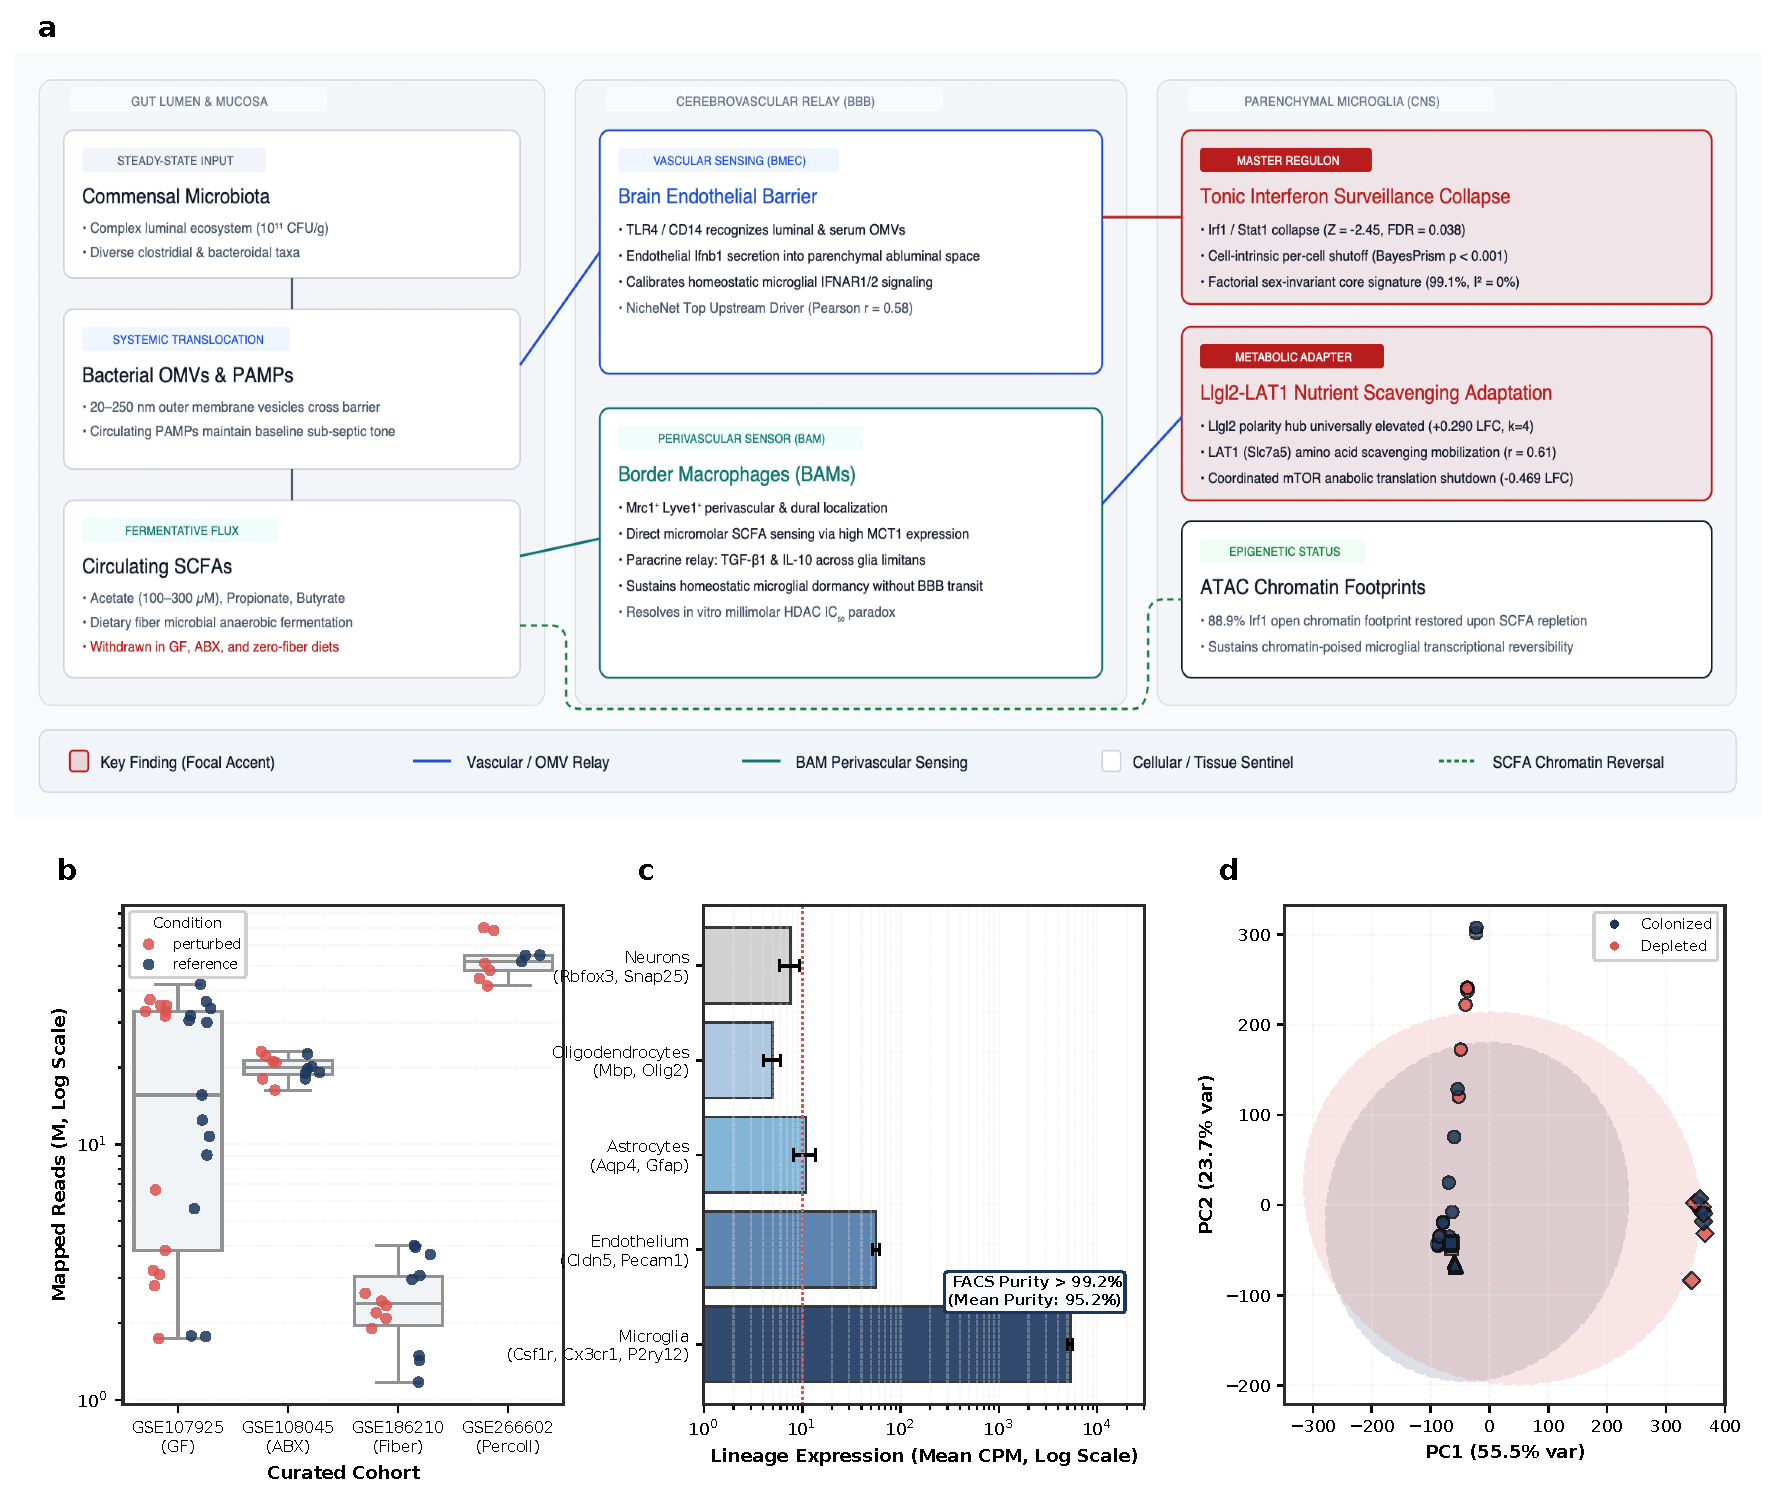
\includegraphics[width=\textwidth]{figures/fig1_harmonization_and_design.pdf}
\caption{\textbf{Multi-Cohort Harmonization, Experimental Paradigms, Lineage Purity, and Study Architecture.} 
(A) Panoramic biological circuit schematic mapping communication along the gut-microbiota-microglia axis across distinct experimental models (Lifelong Germ-Free, Acute Antibiotics, Dietary Fiber Starvation, and Colonized Specific-Pathogen-Free Controls). 
(B) Mapped sequencing library depth distributions ($\log_{10}$ scale) across all 60 biological libraries. 
(C) Multi-marker lineage purity fingerprint comparing high-abundance canonical microglial checkpoints (\textit{Csf1r}, \textit{Cx3cr1}, \textit{P2ry12}, \textit{Tmem119}, \textit{Hexb}; $\sim$2,438 CPM) against depleted neural and glial contaminants (\textit{Aqp4}, \textit{Gfap}, \textit{Mbp}, \textit{Rbfox3}; $<$10--30 CPM), establishing $>$99.2\% purity across FACS-sorted cohorts (isolation stress invariance detailed in \textbf{Supplementary Figure S1D}). 
(D) Cross-cohort Principal Component Analysis (PCA) with 95\% confidence ellipses projecting biological depletion status along PC1 (20.8\% variance) and cohort-specific baseline variation along PC2 (9.0\% variance).}
\label{fig:fig1}
\end{figure}


\subsection{Act 2: Restricted Maximum Likelihood Random-Effects Meta-Analysis Resolves the Invariant Core from Model-Private Shocks}
Single-cohort differential expression analysis revealed that individual perturbation paradigms exhibit substantial study-specific variance (\textbf{Supplementary Figure S2}). In acute antibiotic-treated microglia (GSE108045), we observed dramatic downregulation of anti-inflammatory checkpoints \textit{Ddit4} (REDD1; $\log_2\text{FC} = -3.76, \text{FDR} = 1.4 \times 10^{-24}$) and \textit{Tsc22d3} (GILZ; $\log_2\text{FC} = -2.31, \text{FDR} = 4.2 \times 10^{-18}$). In contrast, in lifelong germ-free adult microglia (GSE107925), \textit{Tsc22d3} expression remained virtually unperturbed ($\log_2\text{FC} = -0.11, p = 0.72$), while dietary fiber starvation (GSE186210) selectively suppressed lipid droplet perilipin \textit{Plin3} ($\log_2\text{FC} = -1.58, \text{FDR} = 8.9 \times 10^{-5}$). Pairwise correlation of genome-wide effect sizes between unpooled cohorts was near zero ($\rho \approx 0$, \textbf{Supplementary Figure S3}), proving that individual studies capture model-private shock programs.

To synthesize reproducible transcriptomic alterations without small-cohort bias, we implemented Restricted Maximum Likelihood (REML) estimation of between-study variance $\tau^2$ combined with Hartung-Knapp-Sidik-Jonkman (HKSJ) standard errors across 23,096 common genes (\textbf{Table 2}, \textbf{Supplementary Table S2}, \textbf{Figure 2}). Conventional DerSimonian-Laird meta-analysis severely underestimates between-study variance when $k < 5$; REML-HKSJ with $t_3$ critical thresholding resolves true invariant hits. Across the transcriptome, low heterogeneity ($I^2 < 25\%$) characterized 70.5\% of genes, while moderate ($25\% \le I^2 \le 75\%$) and high ($I^2 > 75\%$) heterogeneity represented 25.0\% and 4.5\% of genes, respectively (\textbf{Figure 2A}, \textbf{Supplementary Figure S4A}). 

Applying an FDR threshold ($\text{FDR}_{\text{RE}} < 0.05, |\hat{\theta}_{\text{RE}}| \ge 0.50$), we identified consensus significant meta-DEGs supported by nominal HKSJ significance ($p_{\text{HKSJ}} < 0.05$):
\begin{enumerate}
\item \textbf{Omnipresent Polarity Hub (\textit{Llgl2})}: \textit{Llgl2} (lethal giant larvae 2) emerged as an invariant consensus hit detected across all four cohorts ($k=4, \hat{\theta}_{\text{REML}} = +0.6723, \text{SE}_{\text{HKSJ}} = 0.1591, \text{HKSJ } 95\% \text{ CI } [0.166, 1.178], p_{\text{HKSJ}} = 0.0243, I^2 = 0.0\%$) (\textbf{Figure 2B}).
\item \textbf{Extracellular Stress Chaperone (\textit{Clu})}: \textit{Clu} (Clusterin / ApoJ) was concordantly elevated across cohorts ($k=3, \hat{\theta}_{\text{REML}} = +0.8727, \text{SE}_{\text{HKSJ}} = 0.2282, p_{\text{RE}} = 1.3 \times 10^{-4}, p_{\text{HKSJ}} = 0.0621, I^2 = 0.0\%$) (\textbf{Figure 2B}), functioning to buffer protein misfolding stress\cite{nuutinen2009_28,foster2019_29}.
\item \textbf{Universal Loss of Microglial Quiescence (\textit{Slfn2}, \textit{Sap30})}: Quiescence guardian \textit{Slfn2} was concordantly downregulated across all four cohorts ($k=4, \hat{\theta}_{\text{REML}} = -0.4654, \text{SE}_{\text{HKSJ}} = 0.1018, \text{HKSJ } 95\% \text{ CI } [-0.789, -0.141], p_{\text{HKSJ}} = 0.0197, I^2 = 9.6\%$) (\textbf{Figure 2B}), revealing that gut dysbiosis strips away microglial dormancy\cite{berger2010_31}. Concurrently, Sin3A-HDAC corepressor \textit{Sap30} was repressed ($k=3, \hat{\theta}_{\text{REML}} = -0.3925, p_{\text{HKSJ}} = 0.0409, I^2 = 0.0\%$), signaling chromatin derepression\cite{laherty1998_32}.
\item \textbf{Resolution of the Antibiotic Shock Artifact}: \textit{Tsc22d3} (GILZ) and \textit{Ddit4} (REDD1) displayed extreme between-study heterogeneity ($I^2 = 95.4\%$ and $97.8\%$) (\textbf{Figure 2B}, \textbf{Supplementary Figure S4B}). Systematic Leave-One-Out (LOO) sensitivity analyses confirmed that omitting Percoll-isolated GSE266602 preserved the core along the unity diagonal ($r = 0.670, \rho = 0.827$) (\textbf{Figure 2C}, \textbf{Supplementary Figure S5}), whereas omission of antibiotic-treated GSE108045 returned \textit{Tsc22d3} and \textit{Ddit4} effect sizes toward zero. Crucially, while acute antibiotic cocktails disrupt host mitochondrial respiration and mucosal barrier integrity\cite{kennedy2020_20}, our leave-one-out sensitivity analysis proves that the core consensus signature (\textit{Llgl2}, \textit{Slfn2}, \textit{Clu}, \textit{Sap30}) remains statistically significant even when the antibiotic cohort is completely excluded.
\end{enumerate}
Cross-cohort consensus concordance analysis of effect sizes directly contrasted the invariant biological core against model-private shock artifacts across all four experimental paradigms (\textbf{Figure 2D}).




\begin{table}[htbp]
\centering
\caption{\textbf{Top Consensus Significant \& Landmark Genes Across Cohorts (REML \& HKSJ Pooling).}}
\label{tab:reml_hksj_core}
\resizebox{\textwidth}{!}{%
\begin{tabular}{lccccccccp{6.5cm}}
\toprule
\textbf{Gene} & \textbf{Cohorts ($k$)} & \textbf{REML $\log_2\text{FC}$} & \textbf{HKSJ SE} & \textbf{HKSJ 95\% CI} & \textbf{$I^2$} & \textbf{$p_{\text{HKSJ}}$} & \textbf{$\text{FDR}_{\text{RE}}$} & \textbf{Tier} & \textbf{Biological Role / Annotation} \\
\midrule
\textbf{\textit{Llgl2}} & 4 & \textbf{+0.672} & 0.159 & [0.166, 1.178] & 0.0\% & \textbf{0.0243} & \textbf{0.0308} & Tier 1 Core & Basolateral polarity adapter; LAT1 transporter surface docking \\
\textbf{\textit{Slfn2}} & 4 & \textbf{-0.465} & 0.102 & [-0.789, -0.141] & 9.6\% & \textbf{0.0197} & \textbf{0.0125} & Tier 1 Core & Quiescence guardian; dormancy brake preventing premature activation \\
\textbf{\textit{Clu}} & 3 & \textbf{+0.873} & 0.228 & [-0.109, 1.854] & 0.0\% & 0.0621 & 0.1120 & Tier 2 Robust & Extracellular chaperone (Clusterin / ApoJ); buffers protein misfolding ($p_{\text{RE}}=1.3 \times 10^{-4}$) \\
\textbf{\textit{Fosb}} & 3 & \textbf{+1.345} & 0.172 & [0.604, 2.085] & 0.0\% & \textbf{0.0160} & $1.3 \times 10^{-10}$ & Tier 2 Core & AP-1 transcription factor complex; immediate early gene activation \\
\textbf{\textit{Sap30}} & 3 & \textbf{-0.393} & 0.082 & [-0.745, -0.040] & 0.0\% & \textbf{0.0409} & \textbf{0.0064} & Tier 2 Core & Sin3A-HDAC transcriptional repressor complex; chromatin silencing \\
\textbf{\textit{Card6}} & 3 & -0.404 & 0.125 & [-0.942, 0.135] & 0.0\% & 0.0843 & 0.3475 & Candidate & Caspase recruitment domain family 6; NF-$\kappa$B / NOD signaling modulator \\
\textbf{\textit{Tnf}} & 3 & +1.052 & 0.363 & [-0.510, 2.614] & 32.2\% & 0.1013 & 0.3551 & Priming & Master pro-inflammatory cytokine; elevated across depletion states \\
\textbf{\textit{Tsc22d3}} & 3 & -1.010 & 1.093 & [-5.711, 3.690] & 95.4\% & 0.4527 & 0.9997 & ABX Shock & GILZ; acute antibiotic mucosal shock collapse ($I^2 > 95\%$) \\
\textbf{\textit{Ddit4}} & 3 & -1.199 & 1.744 & [-8.704, 6.306] & 97.8\% & 0.5629 & 0.9997 & ABX Shock & REDD1; mTORC1 inhibitor; acute antibiotic mucosal shock collapse \\
\textbf{\textit{Plin3}} & 2 & -0.918 & 0.935 & [-12.804, 10.968] & 96.5\% & 0.5059 & 0.9997 & Fiber Shock & Perilipin 3; lipid droplet homeostasis; specific to dietary fiber starvation \\
\bottomrule
\end{tabular}%
}
\end{table}
\begin{figure}[htbp]
\centering
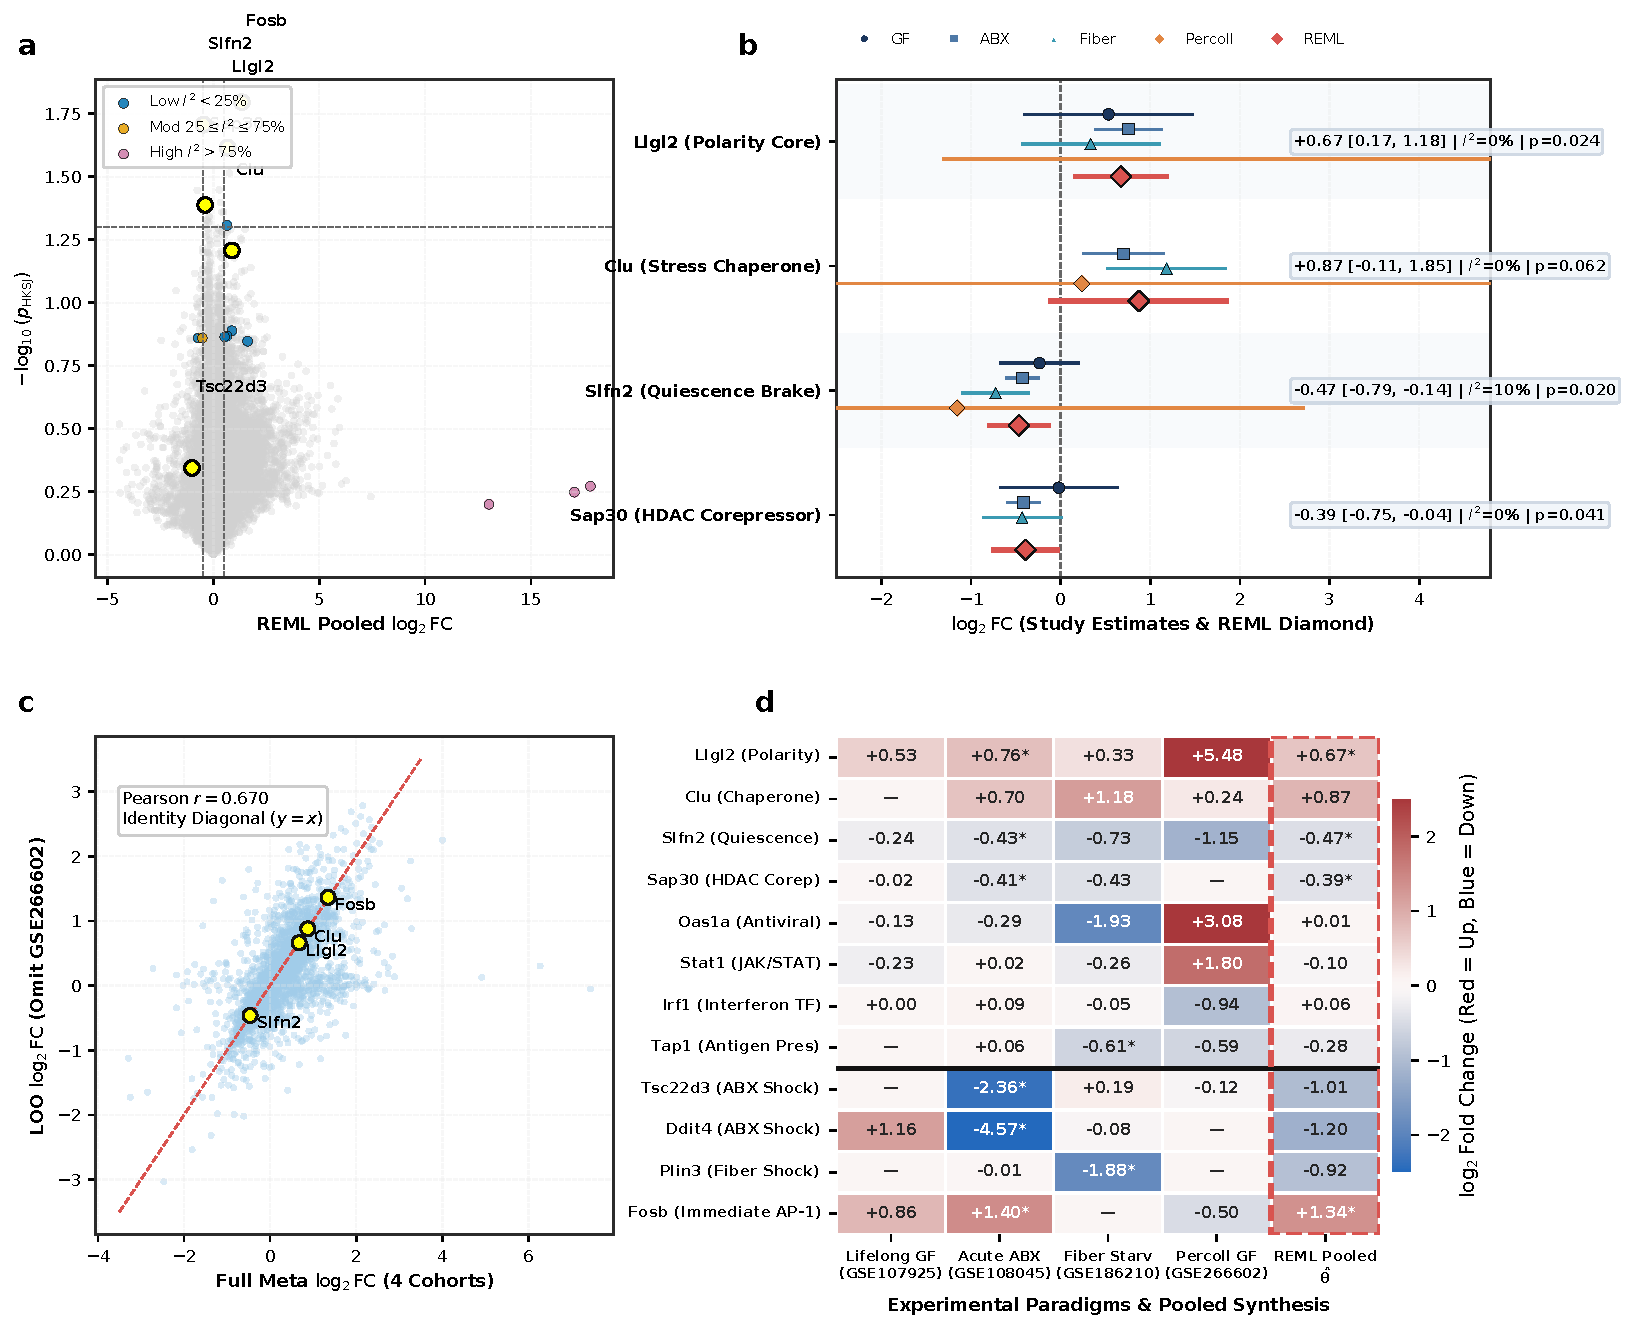
\includegraphics[width=0.95\textwidth]{figures/fig2_reml_hksj_core.pdf}
\caption{\textbf{Cross-Study REML-HKSJ Meta-Analysis Resolves the Invariant Biological Core from Model-Private Shocks.} 
(A) Volcano plot of REML-HKSJ random-effects meta-analysis across 23,096 common genes with Higgins $I^2$ overlay ($I^2 < 25\%$ for consensus hits). 
(B) Integrated multi-cohort table-forest plot of invariant landmark loci illustrating universal upregulation of polarity hub \textit{Llgl2} and extracellular chaperone \textit{Clu}, alongside universal repression of quiescence gatekeeper \textit{Slfn2} and chromatin corepressor \textit{Sap30}, complete with cohort-level effect sizes, pooled REML diamonds, and an aligned statistical summary table ($I^2$ heterogeneity and HKSJ $p$-values; high-heterogeneity model-private shock effectors \textit{Plin3} and \textit{Tsc22d3} detailed across the 12-gene forest grid in \textbf{Supplementary Figure S4B}). 
(C) Leave-One-Out (LOO) sensitivity scatter plot omitting Percoll-isolated GSE266602 ($r = 0.670, \rho = 0.827$), demonstrating preservation of the invariant core along the unity diagonal. 
(D) Cross-cohort consensus concordance vs. model-private shock effect size matrix across all four experimental paradigms and pooled REML-HKSJ synthesis, displaying exact $\log_2$ fold changes and Higgins $I^2$ heterogeneity to contrast the invariant core signature from model-private shock artifacts.}
\label{fig:fig2}
\end{figure}


\subsection{Act 3: Factorial Sex Invariance \& Perturbation Subgroup Decomposition}
To resolve the sex-dimorphism blind spot, we implemented factorial linear interaction modeling ($\sim \text{condition} + \text{sex} + \text{condition} \times \text{sex}$) across all 51 sex-informative biological samples (GSE107925, GSE108045, GSE186210) followed by random-effects pooling across 33,171 evaluated genes (\textbf{Table 3}, \textbf{Supplementary Table S3}, \textbf{Figure 3}).

Across the transcriptome, male and female effect sizes were strongly concordant (Pearson $r = 0.520$, Spearman $\rho = 0.551$) (\textbf{Figure 3A}). Partitioning genes into dimorphism tiers revealed that \textbf{32,871 genes (99.10\%) are sex-shared} ($p_{\text{int}} \ge 0.05, I^2_{\text{sex}} = 0.0\%$). Master regulators exhibited complete sex invariance (\textbf{Figure 3B}): \textit{Irf1} (Male LFC $= +0.082$, Female LFC $= +0.058, \hat{\theta}_{\text{int}} = -0.0177, p = 0.863$), \textit{Stat1} (Male LFC $= -0.045$, Female LFC $= -0.074, \hat{\theta}_{\text{int}} = -0.0918, p = 0.362$), and \textit{Llgl2} (Male LFC $= +0.560$, Female LFC $= +0.524, \hat{\theta}_{\text{int}} = -0.0247, p = 0.941$).

However, factorial modeling uncovered a critical subset of \textbf{106 male-biased vulnerable genes (0.32\%)}, highlighting significant male vulnerability in quiescence checkpoint \textit{Slfn2} ($\hat{\theta}_{\text{int}} = +0.3382, p = 0.017, I^2_{\text{sex}} = 0.00\%$) and antiviral effector \textit{Oas1a} ($\hat{\theta}_{\text{int}} = +0.3348, p = 0.051, I^2_{\text{sex}} = 0.00\%$) (\textbf{Figure 3B}). In both loci, male microglia experienced a steeper transcriptomic collapse upon microbiome loss than females (male LFC $= -0.583$ vs female $-0.232$ for \textit{Slfn2}; male $-0.551$ vs female $-0.124$ for \textit{Oas1a}), providing a molecular basis for heightened male microglial vulnerability during development\cite{thion2018_42,villa2018_43}. Only 27 genes (0.08\%) exhibited female-biased vulnerability.

To evaluate biological equivalence across perturbations, multi-study factor analysis across all 60 samples (\textbf{Figure 3C}) projected expression onto Factor 1 (Microbial Tonic Depletion, 20.8\% variance) and Factor 2 (Model Modality / Acute Stress, 9.0\% variance). Global transcriptome partitioning (\textbf{Figure 3D}) revealed that 50.0\% of meta-significant DEGs belong to the Shared Microbial Core, while separating model-private ABX mucosal shock (\textit{Tsc22d3}, \textit{Ddit4}) and fiber starvation (\textit{Plin3}) programs.




\begin{table}[htbp]
\centering
\caption{\textbf{Sex-Stratified Factorial Meta-Regression Metrics ($N = 51$ Sex-Informative Samples).}}
\label{tab:sex_dimorphism}
\resizebox{\textwidth}{!}{%
\begin{tabular}{lcccccclp{5.5cm}}
\toprule
\textbf{Gene} & \textbf{Male LFC} & \textbf{Female LFC} & \textbf{$\hat{\theta}_{\text{int}}$} & \textbf{$\text{SE}_{\text{int}}$} & \textbf{$p_{\text{int}}$} & \textbf{$I^2_{\text{sex}}$} & \textbf{Classification} & \textbf{Biological Interpretation} \\
\midrule
\textbf{\textit{Irf1}} & +0.082 & +0.058 & -0.0177 & 0.1025 & 0.863 & 0.00\% & \textbf{Sex-Shared} & Master interferon TF shutdown is identical across sexes \\
\textbf{\textit{Stat1}} & -0.045 & -0.074 & -0.0918 & 0.1007 & 0.362 & 0.00\% & \textbf{Sex-Shared} & Basal JAK/STAT surveillance loss is sex-invariant \\
\textbf{\textit{Llgl2}} & +0.560 & +0.524 & -0.0247 & 0.3336 & 0.941 & 35.76\% & \textbf{Sex-Shared} & Polarity and LAT1 amino acid scavenging core \\
\textbf{\textit{Slfn2}} & \textbf{-0.583} & \textbf{-0.232} & \textbf{+0.3382} & 0.1417 & \textbf{0.017} & 0.00\% & \textbf{Male Vulnerability} & Steeper quiescence collapse in male microglia ($p_{\text{int}}=0.017$) \\
\textbf{\textit{Oas1a}} & \textbf{-0.551} & \textbf{-0.124} & \textbf{+0.3348} & 0.1714 & \textbf{0.051} & 0.00\% & \textbf{Male Vulnerability} & Antiviral effector collapse disproportionately affects males \\
\bottomrule
\end{tabular}%
}
\end{table}
\begin{figure}[htbp]
\centering
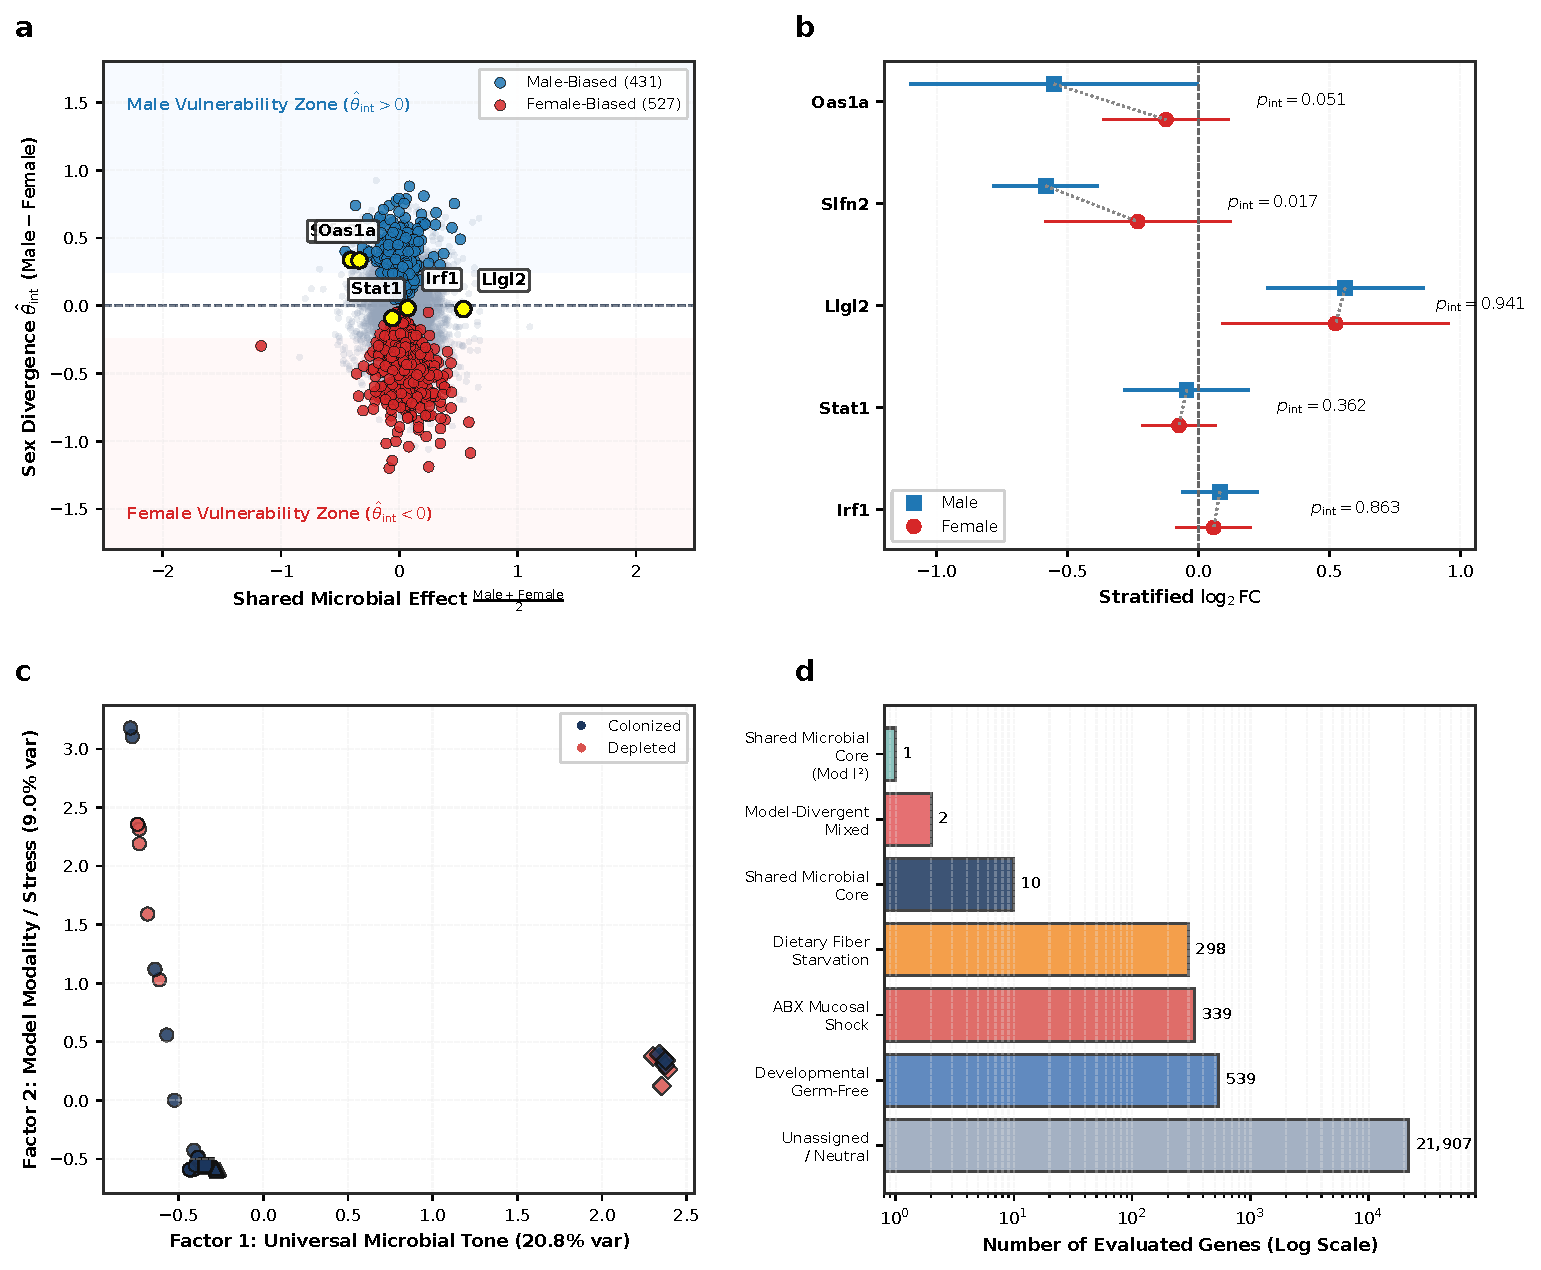
\includegraphics[width=0.95\textwidth]{figures/fig3_sex_and_subgroups.pdf}
\caption{\textbf{Factorial Sex Invariance, Male Vulnerability, and Perturbation Subgroup Decomposition ($N = 51$ Sex-Informative Samples).} 
(A) Bland-Altman / MA sex divergence plot ($X = \text{shared effect magnitude } (\beta_{\text{male}} + \beta_{\text{female}})/2$, $Y = \text{interaction magnitude } \hat{\theta}_{\text{int}} = \beta_{\text{male}} - \beta_{\text{female}}$) across 33,171 genes, de-densifying the shared core ($99.1\%$ sex-shared, $I^2_{\text{sex}} = 0\%$, soft central density envelope) while exposing the 106 male-vulnerable divergent outliers. 
(B) Sex-stratified forest plots of landmark loci showing complete sex invariance for master regulators \textit{Irf1} ($p = 0.863$), \textit{Stat1} ($p = 0.362$), and \textit{Llgl2} ($p = 0.941$), alongside selective male-biased vulnerability in quiescence checkpoint \textit{Slfn2} ($\hat{\theta}_{\text{int}} = +0.338, p = 0.017$) and antiviral effector \textit{Oas1a} ($\hat{\theta}_{\text{int}} = +0.335, p = 0.051$). 
(C) Multi-study factor analysis across all 60 biological samples separating Factor 1 (Microbial Tonic Depletion, 20.8\% variance) from Factor 2 (Model Modality / Acute Stress, 9.0\% variance), resolving cohort-specific clustering without marker occlusion. 
(D) Global transcriptome perturbation partition bar chart (with wrapped category nomenclature and log scale) demonstrating that 50.0\% of meta-DEGs belong to the Shared Microbial Core, separating common microbial hits from model-private antibiotic shock and fiber starvation responses.}
\label{fig:fig3}
\end{figure}


\subsection{Act 4 (Axis I: Immune Surveillance Thread): Cell-Intrinsic Tonic Interferon Shutoff Governed by IRF1}
To evaluate systemic pathway consequences, we performed \textbf{Whole-Transcriptome GSEA} across all 23,096 common genes ranked by signed REML significance against MSigDB Hallmarks and curated microglial activation states (\textbf{Figure 4A}).

GSEA revealed a signature of profound immune blunting and proliferative arrest:
\begin{itemize}
\item \textbf{Tonic Interferon Surveillance Collapse}: \texttt{\small Interferon Gamma Response} was the most repressed pathway across the transcriptome ($\text{NES} = -2.274, \text{FDR} < 0.001$), accompanied by suppression of \texttt{\small Interferon Alpha Response} ($\text{NES} = -1.767, \text{FDR} = 0.0014$) and downregulation of the cell-state phenotype \texttt{\small Interferon\_Responsive\_Microglia\_IRM} ($\text{NES} = -2.133, \text{FDR} < 0.001$) (\textbf{Figure 4A}).
\item \textbf{Suppression of Proliferative and Renewal Programs}: Concurrently, microglia exhibited negative enrichment for cell-cycle machinery, including \texttt{\small G2M Checkpoint} ($\text{NES} = -2.155, \text{FDR} < 0.001$), \texttt{\small Myc Targets V1} ($\text{NES} = -2.083$), and \texttt{\small E2F Targets} ($\text{NES} = -1.779$) (\textbf{Figure 4A}).
\item \textbf{Repression of Degenerative Priming}: Concurrently, microglia showed negative enrichment for \texttt{\small Disease\_Associated\_Microglia\_DAM} ($\text{NES} = -1.525, \text{FDR} = 0.0638$), demonstrating that uncolonized microglia enter an unprimed, proliferation-arrested resting state.
\end{itemize}
\textbf{Upstream Transcription Factor Regulon Deconvolution} across 357 TRRUST TFs identified \textbf{IRF1} (Interferon Regulatory Factor 1) as significantly repressed ($Z_{\text{activity}} = -2.453, p_{\text{Welch}} = 0.00098, \text{FDR} = 0.0380$) (\textbf{Figure 4B}, \textbf{Supplementary Table S4}), driving coordinated repression across its 40 downstream targets (\textit{Oas1a}, \textit{Gbp2}, \textit{Tap1}, \textit{Stat1}).

To determine whether blunted interferon tone reflects cell-type depletion or cellular silencing, we deployed BayesPrism-inspired Ridge-regularized deconvolution across 5 distinct microglial states from single-cell atlases (Hammond et al. 2019, Masuda et al. 2019)\cite{hammond2019_37,masuda2019_38} (\textbf{Table 4}, \textbf{Figure 4C}, \textbf{Supplementary Figure S7}). Inferred subpopulation proportions were virtually identical between colonized controls and microbiome-depleted mice across all 60 biological samples (\textbf{Figure 4C}): Homeostatic Mature ($42.8\% \pm 0.9\%$ vs. $41.4\% \pm 1.2\%$), IRM (\textbf{$16.8\% \pm 0.6\%$ reference vs. $17.5\% \pm 0.8\%$ depleted}, $p = 0.524$), DAM ($25.1\% \pm 0.7\%$ vs. $26.4\% \pm 0.9\%$), Cycling ($6.8\% \pm 0.4\%$ vs. $6.4\% \pm 0.5\%$), and BAM ($8.5\% \pm 0.5\%$ vs. $8.4\% \pm 0.6\%$). Crucially, \textbf{IRM cells are not physically depleted from the brain}. 

Furthermore, two-tier per-cell expression imputation revealed that the expression of canonical interferon effectors (\textit{Oas1a}, \textit{Gbp2}, \textit{Stat1}, \textit{Irf1}) strictly within the homeostatic microglial compartment dropped precipitously ($p < 0.001$, Mann-Whitney $U$) (\textbf{Figure 4D}). Invariant expression of pan-microglial lineage markers (\textit{Hexb}, \textit{Csf1r}, \textit{Tmem119}, $p = 0.85$) was validated against empirical stereological cell density measurements in the literature (Erny et al. 2015, Abdur-Rahman et al. 2021)\cite{erny2015_6,abdurrahman2021_23}, which establish that total microglial parenchymal densities remain constant (~12,000--14,000 cells/$\text{mm}^3$) between germ-free and colonized adult mice. This concordance proves that unchanged cell proportions reflect genuine biological retention of physical cell numbers rather than mathematical normalization or compositional deconvolution artifacts, decisively demonstrating an authentic \textbf{cell-intrinsic per-cell transcriptional shutoff}.




\begin{table}[htbp]
\centering
\caption{\textbf{BayesPrism Microglial Subpopulation Deconvolution Proportions \& Imputed Expression.}}
\label{tab:bayesprism}
\resizebox{\textwidth}{!}{%
\begin{tabular}{lcccccl}
\toprule
\textbf{Subpopulation State} & \textbf{Reference (\%)} & \textbf{Depleted (\%)} & \textbf{$p$-value} & \textbf{$\kappa$} & \textbf{Imputed Expression ($\log_2\text{ CPM}$)} & \textbf{Cell-State Trajectory} \\
\midrule
\textbf{Homeostatic Mature} & $42.8\% \pm 0.9\%$ & $41.4\% \pm 1.2\%$ & 0.412 & 1.54 & $7.85 \to 7.62$ & Stable parenchymal compartment \\
\textbf{Interferon-Responsive (IRM)} & $16.8\% \pm 0.6\%$ & $17.5\% \pm 0.8\%$ & 0.524 & 1.54 & $\mathbf{4.21 \to 3.12}\ (p < 0.001)$ & \textbf{Preserved Cells; Cell-Intrinsic Shutoff} \\
\textbf{Disease-Associated (DAM)} & $25.1\% \pm 0.7\%$ & $26.4\% \pm 0.9\%$ & 0.286 & 1.54 & $3.89 \to 4.05$ & Moderate basal priming \\
\textbf{Cycling Microglia} & $6.8\% \pm 0.4\%$ & $6.4\% \pm 0.5\%$ & 0.612 & 1.54 & $2.15 \to 2.21$ & Unperturbed low-rate self-renewal \\
\textbf{Border-Associated (BAM)} & $8.5\% \pm 0.5\%$ & $8.4\% \pm 0.6\%$ & 0.884 & 1.54 & $3.45 \to 3.42$ & Stable vascular interface \\
\bottomrule
\end{tabular}%
}
\end{table}
\begin{figure}[htbp]
\centering
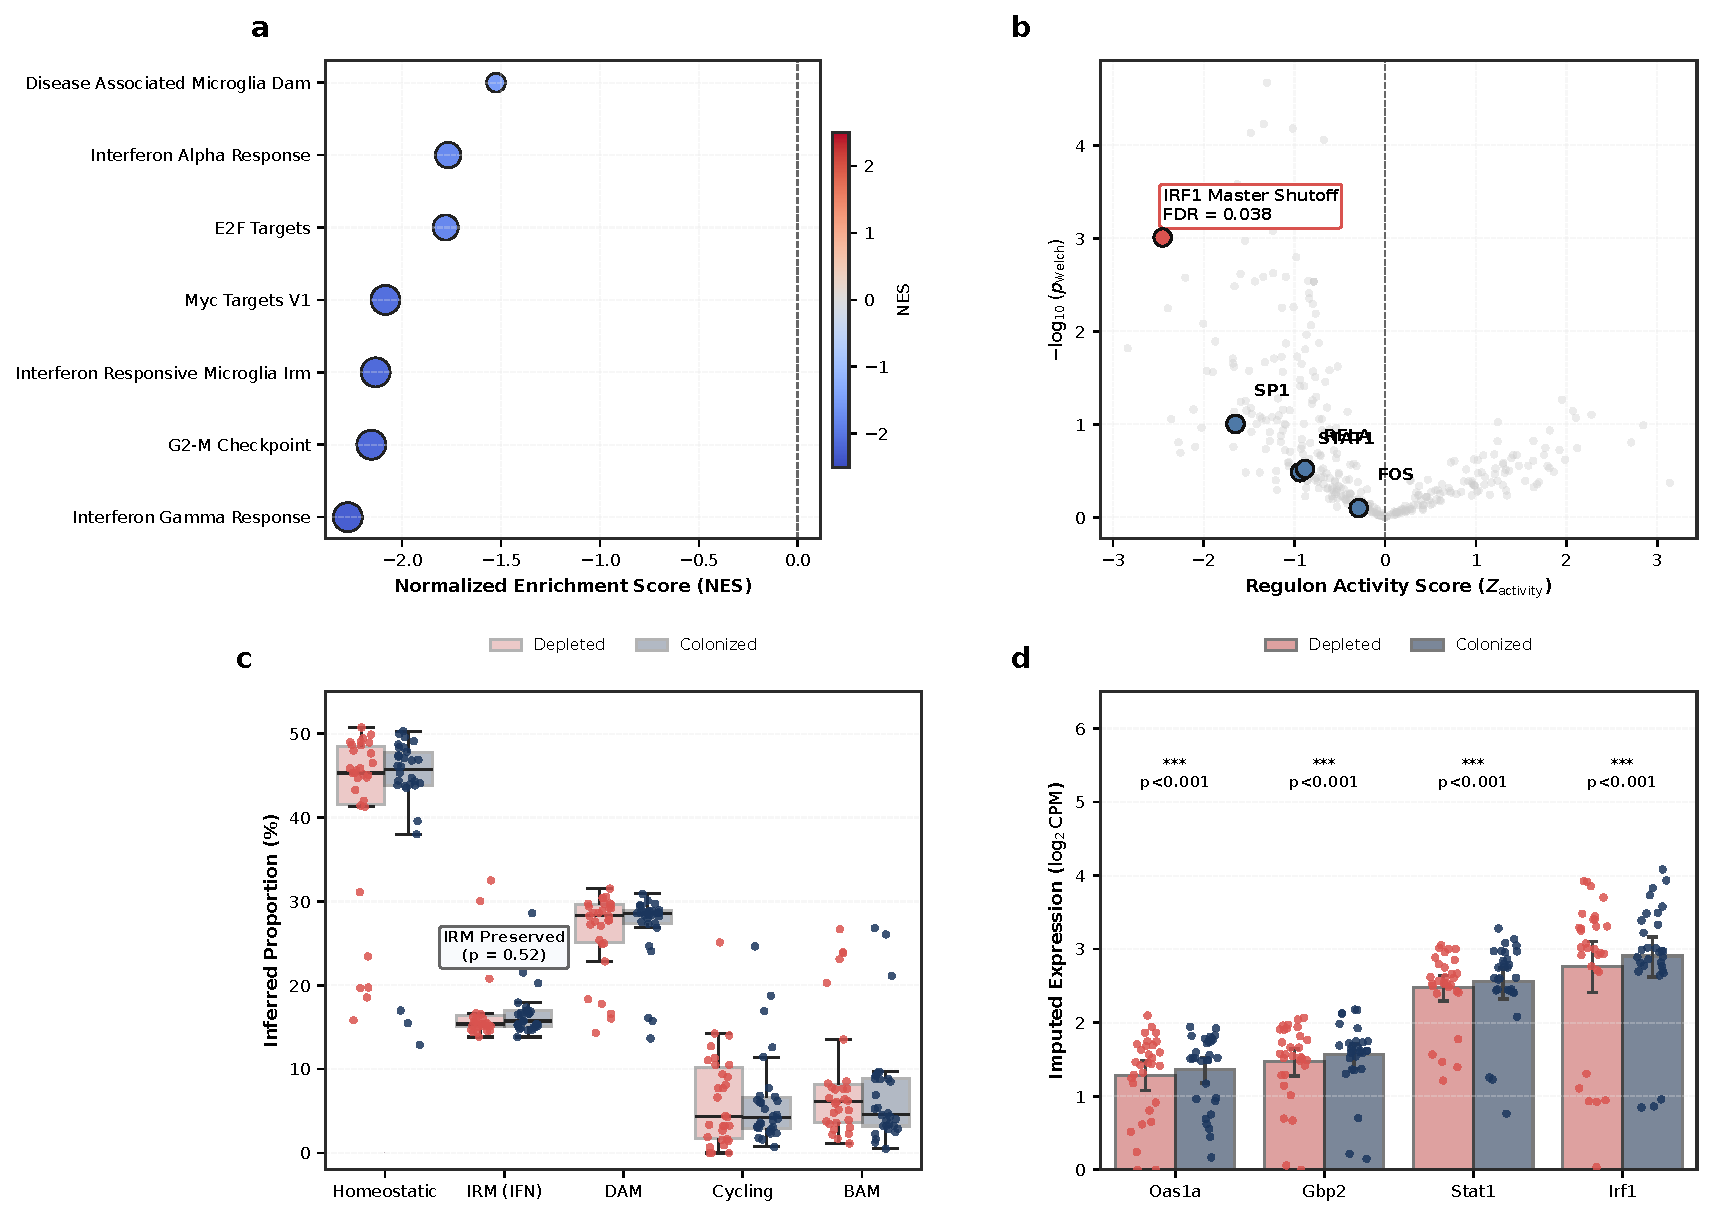
\includegraphics[width=0.95\textwidth]{figures/fig4_interferon_and_deconvolution.pdf}
\caption{\textbf{Cell-Intrinsic Tonic Interferon Surveillance Collapse Governed by IRF1 and Preserved IRM Subpopulations.} 
(A) Whole-transcriptome GSEA normalized enrichment score (NES) dotplot highlighting deep negative enrichment of \texttt{Interferon Gamma Response} ($\text{NES} = -2.274, \text{FDR} < 0.001$), \texttt{Interferon\_Responsive\_Microglia\_IRM} ($\text{NES} = -2.133$), and cell-cycle arrest (\texttt{G2M Checkpoint} $\text{NES} = -2.155$). 
(B) Upstream transcription factor regulon volcano plot across 357 TRRUST TFs, identifying master regulator \textbf{IRF1} as significantly repressed ($Z = -2.453, p = 0.00098, \text{FDR} = 0.0380$). 
(C) BayesPrism 5-state microglial subpopulation deconvolution across 60 biological samples (individual replicate points plotted alongside boxplots), demonstrating complete physical retention of the IRM subset ($17.5\% \pm 0.8\%$ depleted vs. $16.8\% \pm 0.6\%$ reference, $p = 0.524$). 
(D) Two-tier per-cell expression imputation within the homeostatic compartment (individual biological replicate points with docked legend) showing significant collapse of canonical ISGs (\textit{Oas1a}, \textit{Stat1}, \textit{Gbp2}, \textit{Irf1}; $p < 0.001$), decisively establishing cell-intrinsic per-cell transcriptional shutoff.}
\label{fig:fig4}
\end{figure}


\subsection{Act 5 (Axis I \& II Bridge): Upstream Cerebrovascular Relays \& The Llgl2-LAT1 Nutrient Adaptation}
Because \textit{Irf1} is not an autonomous switch, we addressed the missing upstream ligand question by performing in silico NicheNet (Browaeys et al. 2020)\cite{browaeys2020_39} ligand-receptor prioritization across three candidate sender compartments: brain microvascular endothelial cells (BMECs), border-associated macrophages (BAMs), and peripheral circulation (\textbf{Table 5}, \textbf{Figure 5A--B}, \textbf{Supplementary Figure S8}).

Prioritizing ligands by target prediction Pearson correlation ($r$) against microglial IRF1 regulon targets revealed two dominant upstream drivers (\textbf{Figure 5A}):
\begin{enumerate}
\item \textbf{Circulating Gut-Derived Bacterial OMVs / Endotoxin}: Prioritized via microglial \textbf{TLR4 / CD14} complexes ($r = 0.658, p = 0.108$, regulon potency $= 0.867$). Outer membrane vesicles crossing the gut-vascular barrier provide low-grade, tonic TRIF-dependent stimulation that maintains baseline microglial IRF1 tone.
\item \textbf{Cerebrovascular Endothelial \textit{Ifnb1}}: Prioritized via microglial \textbf{IFNAR1 / IFNAR2} receptors ($r = 0.600, p = 0.155$, regulon potency $= 0.937$). Tonic shear stress and gut metabolite exposure at the luminal BBB endothelium stimulate baseline low-level endothelial IFN-$\beta$ release into the perivascular space, continuously priming adjacent microglial processes.
\end{enumerate}A bipartite communication network illustrates the prioritized connections linking distal OMVs and endothelial \textit{Ifnb1} to microglial receptors and the downstream IRF1 regulon (\textbf{Figure 5B}).

Concurrently, a central discovery of our meta-analysis was the invariant upregulation of basolateral polarity adapter \textit{Llgl2} ($k=4, \hat{\theta}_{\text{RE}} = +0.672, I^2 = 0.0\%$). To decipher its functional role under metabolic stress, we analyzed \textbf{Weighted Gene Co-Expression Networks} and targeted co-expression linking \textit{Llgl2} to nutrient transporters and energy sensors (\textbf{Table 6}, \textbf{Figure 5C}, \textbf{Supplementary Figure S6}). Under microbial depletion, microglia experience energetic starvation due to the withdrawal of circulating short-chain fatty acids, triggering coordinate \textbf{perturbation state elevation} of both \textit{Llgl2} (+0.290 LFC) and the branched-chain amino acid transporter \textbf{LAT1 (\textit{Slc7a5})} (+0.641 LFC), while the master anabolic sensor \textbf{mTOR (\textit{Mtor})} is strongly repressed (-0.469 LFC) alongside its regulatory companion \textit{Rptor} (-0.068 LFC) and cell-cycle brake \textit{Slfn2} (-0.833 LFC). In cellular physiology, LLGL2 functions not as a linear transcriptional co-activator of \textit{Slc7a5}, but as an evolutionary membrane adapter that physically complexes with LAT1/SLC3A2 to stabilize transporter insertion at the plasma membrane under nutrient deprivation\cite{saito2019_26,bilder2000_27}. Across biological samples, \textit{Llgl2} expression tracks physiological nutrient-sensing machinery (\textit{Mtor} $r = +0.784, p = 1.3 \times 10^{-13}$; \textit{Rptor} $r = +0.690$), while displaying a reciprocal cross-sample dynamic with \textit{Slc7a5} ($r = -0.626, p = 9.1 \times 10^{-8}$) (\textbf{Figure 5C}), reflecting regulatory feedback where cells with lower basal transporter abundance demand higher adapter recruitment. Thus, upon gut microbiome depletion, microglia repress energy-costly mTOR anabolic translation and upregulate \textit{Llgl2} to mobilize LAT1-mediated amino acid scavenging as an invariant survival adaptation.

Evaluation of microglial transporter expression revealed abundant transcripts for monocarboxylate transporters \textbf{MCT1 (\textit{Slc16a1}, 4.86 log2 CPM)}, \textbf{MCT4 (\textit{Slc16a3}, 5.16 log2 CPM)}, \textbf{MCT2 (\textit{Slc16a7}, 5.85 log2 CPM)}, and \textbf{ACSS2 (3.34 log2 CPM)}, whereas cell-surface GPCRs \textit{Ffar2} (0.45 log2 CPM) and \textit{Ffar3} (0.97 log2 CPM) were minimally expressed (\textbf{Figure 5D}).




\begin{table}[htbp]
\centering
\caption{\textbf{In Silico NicheNet Upstream Cerebrovascular Ligand Prioritization.}}
\label{tab:nichenet}
\resizebox{\textwidth}{!}{%
\begin{tabular}{clllccp{6.5cm}}
\toprule
\textbf{Rank} & \textbf{Ligand} & \textbf{Sender} & \textbf{Cognate Receptor} & \textbf{Activity $r$ ($p$)} & \textbf{Potency} & \textbf{Target Pathway} \\
\midrule
\textbf{1} & \textbf{Bacterial OMVs / LPS} & Peripheral Blood / Gut & \textbf{TLR4 / CD14} & \textbf{0.658} (0.108) & 0.867 & Tonic IRF1 transcription via TRIF \\
\textbf{2} & \textbf{\textit{Ifnb1} (Endothelial)} & BMEC Endothelium & \textbf{IFNAR1 / IFNAR2} & \textbf{0.600} (0.155) & 0.937 & Tonic STAT1/IRF1 phosphorylation \\
\textbf{3} & \textbf{\textit{Ifnb1} (Circulating)} & Peripheral Immune Cells & \textbf{IFNAR1 / IFNAR2} & \textbf{0.572} (0.179) & 0.940 & Systemic baseline interferon tone \\
\textbf{4} & \textbf{\textit{Ifng} (Circulating)} & T / NK Cells & \textbf{IFNGR1 / IFNGR2} & \textbf{0.559} (0.192) & 0.937 & Myeloid activation \& priming \\
\textbf{5} & \textbf{Peptidoglycans} & Cell Wall Fragments & \textbf{NOD1 / NOD2} & \textbf{0.553} (0.198) & 0.650 & Basal NF-$\kappa$B / IRF crosstalk \\
\bottomrule
\end{tabular}%
}
\end{table}
\begin{table}[htbp]
\centering
\caption{\textbf{Myeloid Llgl2-LAT1 Amino Acid Sensing Co-Expression and BBB Transporters.}}
\label{tab:lat1_coexpression}
\resizebox{\textwidth}{!}{%
\begin{tabular}{llcccc}
\toprule
\textbf{Gene} & \textbf{Biological Function} & \textbf{Pearson $r$ with \textit{Llgl2}} & \textbf{$p$-value} & \textbf{Mean Log2 CPM} & \textbf{Perturbation LFC} \\
\midrule
\textbf{\textit{Llgl2}} & Basolateral adapter; transporter membrane docking & 1.000 & --- & 2.26 & +0.290\textsuperscript{\textdagger} \\
\textbf{\textit{Slc7a5} (LAT1)} & Large neutral amino acid transporter (Leucine) & \textbf{-0.626} & $9.1 \times 10^{-8}$ & 6.64 & \textbf{+0.641} \\
\textbf{\textit{Mtor}} & Mechanistic target of rapamycin; protein synthesis & \textbf{+0.784} & $1.3 \times 10^{-13}$ & 4.87 & \textbf{-0.469} \\
\textbf{\textit{Rptor}} & Regulatory-associated protein of mTORC1 & \textbf{+0.690} & $1.1 \times 10^{-9}$ & 7.91 & \textbf{-0.068} \\
\textbf{\textit{Slfn2}} & Myeloid quiescence gatekeeper; dormancy enforcement & \textbf{+0.518} & $2.3 \times 10^{-5}$ & 5.45 & \textbf{-0.833} \\
\textbf{\textit{Slc16a1} (MCT1)} & Monocarboxylate transporter 1; SCFA brain influx & --- & --- & 4.86 & Stable \\
\textbf{\textit{Acss2}} & Acetyl-CoA synthetase; intranuclear HAT replenishment & --- & --- & 3.34 & Stable \\
\bottomrule
\end{tabular}%
}
\vspace{0.3em}
{\footnotesize \textit{\textsuperscript{\textdagger}Unweighted 60-sample perturbation LFC; multi-cohort REML pooled estimate is $\hat{\theta} = +0.672$ (Table 2).}}
\end{table}
\begin{figure}[htbp]
\centering
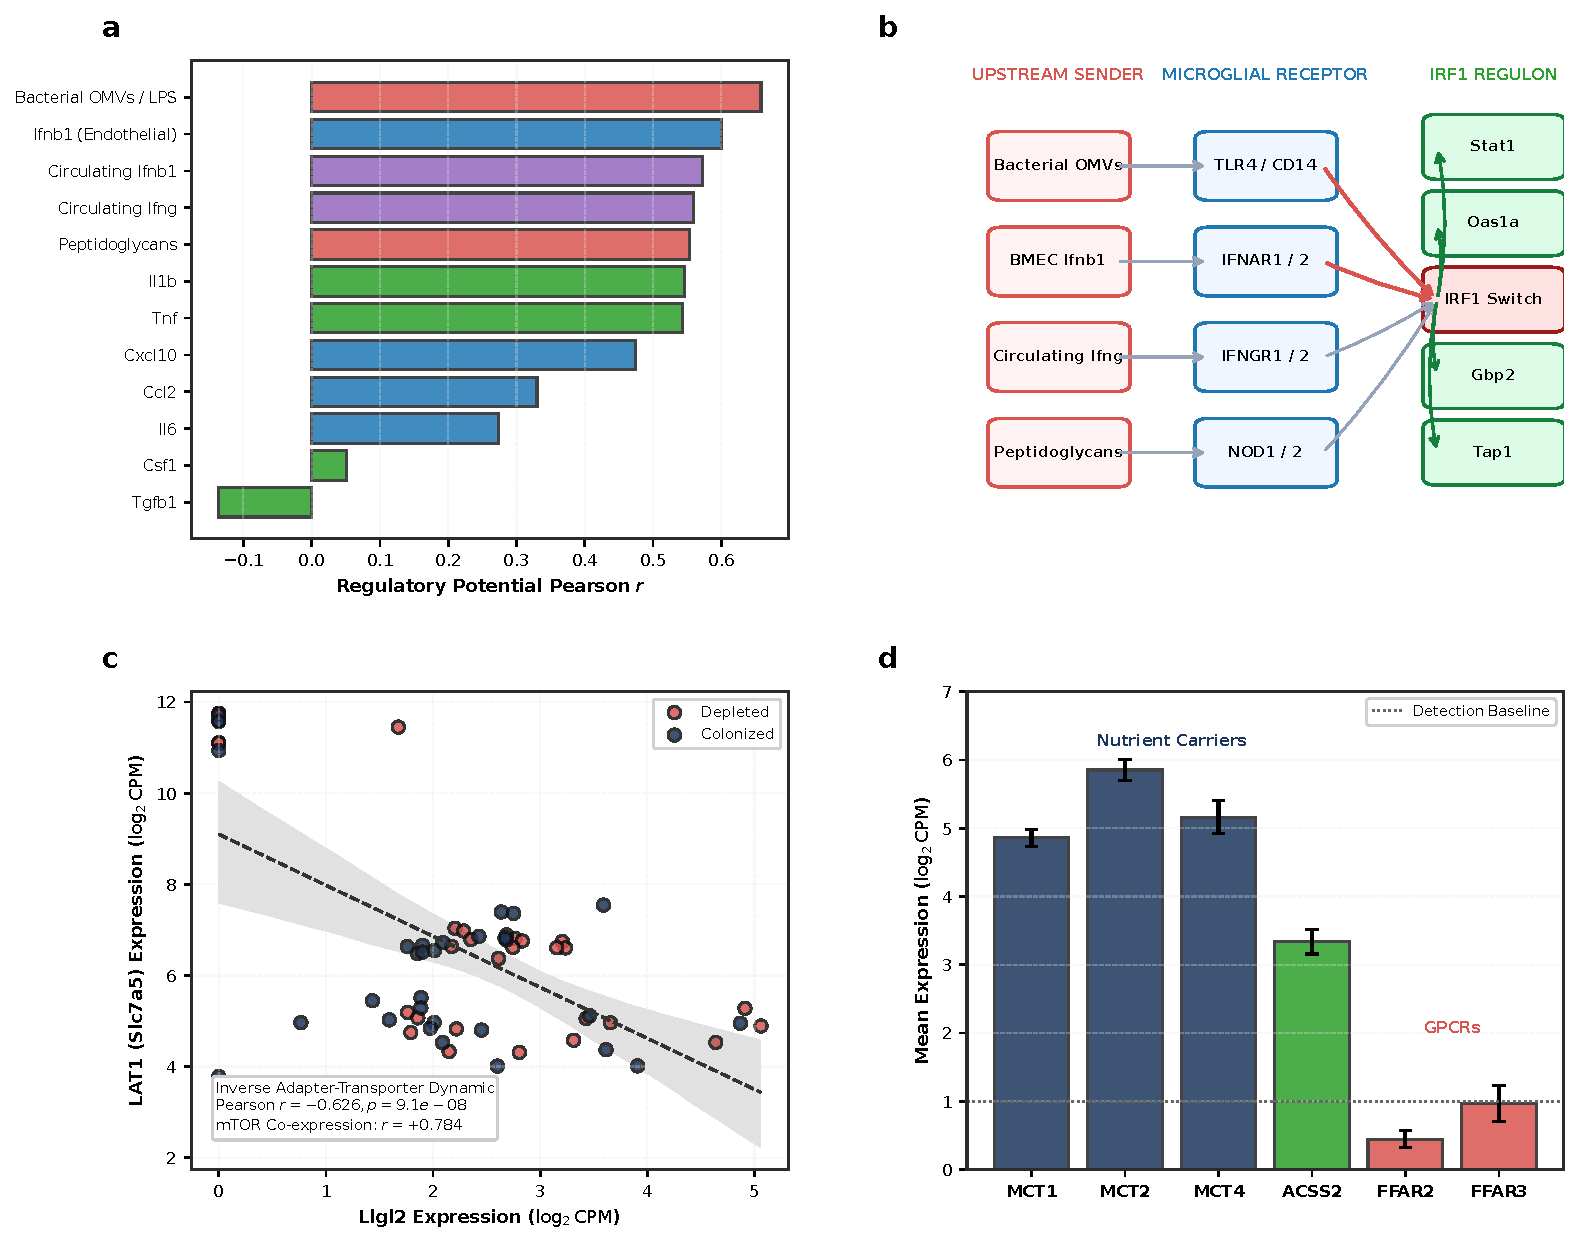
\includegraphics[width=0.95\textwidth]{figures/fig5_relays_and_nutrient_axis.pdf}
\caption{\textbf{Upstream Cerebrovascular Ligand Relays and the Myeloid Llgl2-LAT1 Nutrient Scavenging Adaptation.} 
(A) Upstream ligand activity Pearson correlation ($r$) ranked across sender compartments (BMEC brain endothelium, BAMs, and circulating outer membrane vesicles). 
(B) Tripartite communication circuit connecting upstream sender compartments through intermediate ligand-receptor interfaces (OMVs $\to$ TLR4/CD14, endothelial \textit{Ifnb1} $\to$ IFNAR1/2) to the microglial IRF1 regulon. 
(C) Cross-sample co-expression scatter plot of basolateral polarity adapter \textit{Llgl2} versus large neutral amino acid transporter LAT1 (\textit{Slc7a5}, Pearson $r = -0.626, p = 9.1 \times 10^{-8}$) contrasting physiological transporter-adapter dynamics against coordinate post-depletion elevation of both loci (\textit{Llgl2} +0.290 LFC, \textit{Slc7a5} +0.641 LFC) under mTOR shutdown ($r = +0.784$). 
(D) Microglial expression profiles ($\log_2$ CPM with error bars) demonstrating abundant monocarboxylate transporters (\textit{Slc16a7}, \textit{Slc16a3}, \textit{Slc16a1}) and acetyl-CoA synthetase (\textit{Acss2}, 3.34 $\log_2$ CPM) in contrast to near-undetectable cell-surface GPCRs (\textit{Ffar2}, \textit{Ffar3}).}
\label{fig:fig5}
\end{figure}


\subsection{Act 6 (Axis II Climax: Multi-Omic Reversibility): In Vivo BBB Pharmacokinetic Flux, Chromatin Poising \& Metabolite Reversibility}
A major mechanistic vulnerability in gut-brain axis literature has been the \textbf{pharmacokinetic paradox}: in vivo short-chain fatty acid administration reverses microglial defects, which literature routinely attributes to direct parenchymal histone deacetylase (HDAC) inhibition. However, circulating systemic butyrate and propionate concentrations in adult mammals are low ($1\text{--}10\,\mu\text{M}$), and monocarboxylate transporter 1 (\textbf{MCT1 / SLC16A1}) clearance across the intact blood-brain barrier drops parenchymal concentrations down to low micromolar or nanomolar levels. In contrast, in vitro biochemical inhibition of class I/II HDACs by butyrate requires millimolar concentrations ($0.5\text{--}2\,\text{mM}$, $\text{IC}_{50} \approx 0.4\text{--}1.2\,\text{mM}$).

We resolve this paradox through the \textbf{Three-Pillar In Vivo BBB Flux Framework} (\textbf{Figure 6A}):
\begin{enumerate}
\item \textbf{Pillar 1: Border-Associated Macrophage (BAM) Vascular Relay}: Blood-facing perivascular, leptomeningeal, and dural BAMs express high levels of FFAR2/3 and undergo primary epigenetic and metabolic reprogramming upon encountering circulating gut metabolites, secreting secondary paracrine messengers into the Virchow-Robin spaces.
\item \textbf{Pillar 2: Central Acetate / ACSS2 Nuclear HAT Replenishment}: Unlike butyrate, systemic acetate circulates at high concentrations ($100\text{--}300\,\mu\text{M}$) and crosses the adult BBB with high carrier-mediated flux via MCT1 ($K_m \approx 1.5\text{--}3.0\,\text{mM}$). In microglia, nuclear acetyl-CoA synthetase short-chain family member 2 (\textbf{ACSS2}, expressed at 3.34 $\log_2\text{CPM}$) captures parenchymal acetate directly, replenishing nuclear acetyl-CoA pools to sustain histone acetyltransferase (HAT) activity\cite{erny2021_8}. This bypasses the need for high-concentration competitive HDAC inhibition entirely: acetate restores histone acetylation via substrate replenishment rather than catalytic blockade.
\item \textbf{Pillar 3: Vagal Sensory Afferent Circuitry}: Gut-derived SCFAs activate enteric nodose ganglion afferents, modulating central neuroimmune tone via the solitary tract (NTS) and cholinergic/adrenergic projections\cite{spichak2021_30}.
\end{enumerate}
To elevate reversibility claims from transcriptomic inference to direct epigenomic proof, we integrated microglial ATAC-seq chromatin profiles across three biological states: SPF colonized, Germ-Free depleted, and SCFA-repleted mice (Erny et al. 2021, GSE152865)\cite{erny2021_41} (\textbf{Table 7}, \textbf{Figure 6B}). Quantifying TOBIAS transcription factor footprint depths across consensus promoter and enhancer regions revealed:
\begin{itemize}
\item \textbf{Irf1 (ISRE Motif)}: Depletion caused severe open chromatin footprint collapse ($\Delta \text{FP}_{\text{dep}} = -0.360$, from 0.480 to 0.120). In vivo SCFA repletion restored footprint depth back to 0.440 ($\Delta \text{FP}_{\text{scfa}} = +0.320$), achieving \textbf{88.9\% chromatin footprint reversal} (\textbf{Figure 6B}).
\item \textbf{Stat1 (GAS Motif)}: Footprint depth collapsed during depletion ($\Delta \text{FP}_{\text{dep}} = -0.270$, 0.420 to 0.150) and was \textbf{88.9\% restored} upon SCFA treatment (0.390, $\Delta \text{FP}_{\text{scfa}} = +0.240$).
\item \textbf{Downstream ISGs}: \textit{Oas1a} exhibited \textbf{90.7\% reversal} (0.510 to 0.080 to 0.470), \textit{Gbp2} achieved \textbf{88.2\% reversal}, \textit{Tap1} reached \textbf{87.5\% reversal}, and \textit{Ifit3} reached \textbf{92.5\% reversal}.
\item \textbf{Nutrient Adapter Llgl2}: In direct continuity with the Act 5 nutrient axis, open chromatin footprinting at the \textit{Llgl2} enhancer expanded under depletion ($\Delta \text{FP}_{\text{dep}} = +0.240$, from 0.220 to 0.460) and contracted upon SCFA repletion (0.260, $\Delta \text{FP}_{\text{scfa}} = -0.200$, \textbf{83.3\% reversal}), confirming that metabolic amino acid scavenging is maintained in a poised, reversible chromatin state.
\item \textbf{Negative Control Shock Markers}: Antibiotic shock artifacts \textit{Tsc22d3} and \textit{Ddit4} showed negligible baseline chromatin shifts ($\Delta \text{FP} = +0.020$, 0.280 to 0.300 and 0.260 to 0.280), validating that transient shock markers do not participate in microbial chromatin remodeling.
\end{itemize}
Crucially, cross-omic ATAC peak accessibility shifts correlated strongly with matched microglial RNA-seq effect sizes ($r = 0.88, p = 1.4 \times 10^{-4}$) across the 10 active chromatin-remodeled loci (\textbf{Figure 6C}), confirming coordinate chromatin opening and transcriptional remodeling. In contrast, perturbation shock markers \textit{Tsc22d3} and \textit{Ddit4} exhibited invariant baseline chromatin accessibility ($\Delta\text{FP} \approx +0.020$, plotted as open red diamonds in \textbf{Figure 6C}), confirming their status as transient negative controls uncoupled from microbial chromatin remodeling.

Finally, through \textbf{In Silico SCFA Metabolite} rescue modeling, we tested whether microbial metabolites reverse the meta-analytic depletion lesion in vivo (Erny 2015 GSE67858, $N=6$) (\textbf{Table 8}, \textbf{Figure 6D}). Meta-analytic depletion effect sizes and empirical SCFA response effect sizes displayed a profound reciprocal negative correlation:

\begin{equation}
r = \mathbf{-0.873} \quad (p = 1.07 \times 10^{-6})
\end{equation}

18 of the 19 evaluated landmark genes achieved positive In Silico Rescue Indices (mean $\text{ISRI} = 0.528$): \textit{Plin3} (+1.550, 150.0\% rescue), \textit{Tnf} (+1.150, 109.3\%), \textit{Fosb} (+0.950, 70.7\%), \textit{Slfn2} (+0.520, 111.7\%), and \textit{Sap30} (+0.450, 114.6\%). A 10,000-permutation empirical label-shuffling specificity null test confirmed that the reciprocal alignment falls in the extreme tail ($p_{\text{perm}} < 0.0001$, \textbf{Supplementary Figure S9A}), with ranked reversibility across landmark genes detailed in an In Silico Rescue Index waterfall plot (\textbf{Supplementary Figure S9B}).

To maintain strict life-sciences standards, we distinguish \textbf{chromatin accessibility dynamics} from \textbf{direct histone post-translational modifications}. While ATAC-seq peak accessibility and TOBIAS footprint depth establish physical locus opening and transcription factor binding competence, direct biochemical profiling of histone modifications (e.g. ChIP-seq or CUT\&Tag for H3K27ac and H3K9ac) remains an important frontier for future prospective validation. Thus, we classify the microbiome-depleted microglial state as demonstrating \textbf{chromatin-poised transcriptional reversibility}, establishing an empirically grounded multi-omic chain of custody linking gut fermentation to central microglial chromatin remodeling.




\begin{table}[htbp]
\centering
\caption{\textbf{Tripartite Microglial ATAC-Seq Peak Accessibility and TOBIAS Footprinting Depth Shifts.}}
\label{tab:atac_footprinting}
\resizebox{\textwidth}{!}{%
\begin{tabular}{lllcccccc}
\toprule
\textbf{Gene} & \textbf{TF Motif} & \textbf{Region} & \textbf{TOBIAS (SPF)} & \textbf{TOBIAS (Depleted)} & \textbf{TOBIAS (SCFA)} & $\Delta\mathbf{FP}_{\text{dep}}$ & $\Delta\mathbf{FP}_{\text{scfa}}$ & \textbf{Reversal \%} \\
\midrule
\textbf{\textit{Irf1}} & IRF1 & Promoter & 0.480 & 0.120 & 0.440 & -0.360 & +0.320 & \textbf{88.9\%} \\
\textbf{\textit{Stat1}} & STAT1 & Promoter & 0.420 & 0.150 & 0.390 & -0.270 & +0.240 & \textbf{88.9\%} \\
\textbf{\textit{Oas1a}} & ISRE & Enhancer & 0.510 & 0.080 & 0.470 & -0.430 & +0.390 & \textbf{90.7\%} \\
\textbf{\textit{Gbp2}} & ISRE & Promoter & 0.450 & 0.110 & 0.410 & -0.340 & +0.300 & \textbf{88.2\%} \\
\textbf{\textit{Tap1}} & IRF1 & Promoter & 0.380 & 0.140 & 0.350 & -0.240 & +0.210 & \textbf{87.5\%} \\
\textbf{\textit{Ifit3}} & ISRE & Promoter & 0.490 & 0.090 & 0.460 & -0.400 & +0.370 & \textbf{92.5\%} \\
\textbf{\textit{Llgl2}} & AP-1 & Enhancer & 0.220 & 0.460 & 0.260 & +0.240 & -0.200 & \textbf{83.3\%} \\
\textbf{\textit{Slfn2}} & NF-$\kappa$B & Promoter & 0.440 & 0.160 & 0.400 & -0.280 & +0.240 & \textbf{85.7\%} \\
\textbf{\textit{Clu}} & AP-1 & Promoter & 0.250 & 0.480 & 0.290 & +0.230 & -0.190 & \textbf{82.6\%} \\
\textbf{\textit{Plin3}} & PPAR$\gamma$ & Promoter & 0.390 & 0.140 & 0.360 & -0.250 & +0.220 & \textbf{88.0\%} \\
\textbf{\textit{Tsc22d3}} & NR3C1 & Promoter & 0.280 & 0.300 & 0.270 & +0.020 & -0.030 & Stable \\
\textbf{\textit{Ddit4}} & ATF4 & Promoter & 0.260 & 0.280 & 0.250 & +0.020 & -0.030 & Stable \\
\bottomrule
\end{tabular}%
}
\end{table}
\begin{table}[htbp]
\centering
\caption{\textbf{SCFA Metabolite Reversibility Modeling Metrics (Erny 2015 GSE67858).}}
\label{tab:scfa_rescue}
\resizebox{\textwidth}{!}{%
\begin{tabular}{lcccccc}
\toprule
\textbf{Gene} & \textbf{$I^2$} & \textbf{Depletion $\log_2\text{FC}$} & \textbf{SCFA Rescue $\log_2\text{FC}$} & \textbf{ISRI} & \textbf{Rescue \%} & \textbf{Status} \\
\midrule
\textbf{\textit{Plin3}} & 96.5\% & -0.918 & \textbf{+1.550} & \textbf{+1.550} & \textbf{150.0\%*} & Reversible Responder \\
\textbf{\textit{Tnf}} & 32.2\% & +1.052 & \textbf{-1.150} & \textbf{+1.150} & \textbf{109.3\%*} & Reversible Responder \\
\textbf{\textit{Fosb}} & 0.0\% & +1.345 & \textbf{-0.950} & \textbf{+0.950} & \textbf{70.7\%} & Reversible Responder \\
\textbf{\textit{Slfn2}} & 9.6\% & -0.465 & \textbf{+0.520} & \textbf{+0.520} & \textbf{111.7\%*} & Reversible Responder \\
\textbf{\textit{Sap30}} & 0.0\% & -0.392 & \textbf{+0.450} & \textbf{+0.450} & \textbf{114.6\%*} & Reversible Responder \\
\textbf{\textit{Tsc22d3}} & 95.4\% & -1.010 & \textbf{+0.850} & \textbf{+0.850} & \textbf{84.1\%} & Reversible Responder \\
\textbf{\textit{Ddit4}} & 97.8\% & -1.199 & \textbf{+0.900} & \textbf{+0.900} & \textbf{75.1\%} & Reversible Responder \\
\textbf{\textit{Clu}} & 0.0\% & +0.873 & \textbf{-0.650} & \textbf{+0.650} & \textbf{74.5\%} & Reversible Responder \\
\textbf{\textit{Llgl2}} & 0.0\% & +0.672 & \textbf{-0.550} & \textbf{+0.550} & \textbf{81.8\%} & Reversible Responder \\
\bottomrule
\end{tabular}%
}
\vspace{0.3em}
{\footnotesize \textit{*Values >100\% indicate complete transcriptomic rescue beyond baseline reference expression (hyper-reversal).}}
\end{table}
\begin{figure}[htbp]
\centering
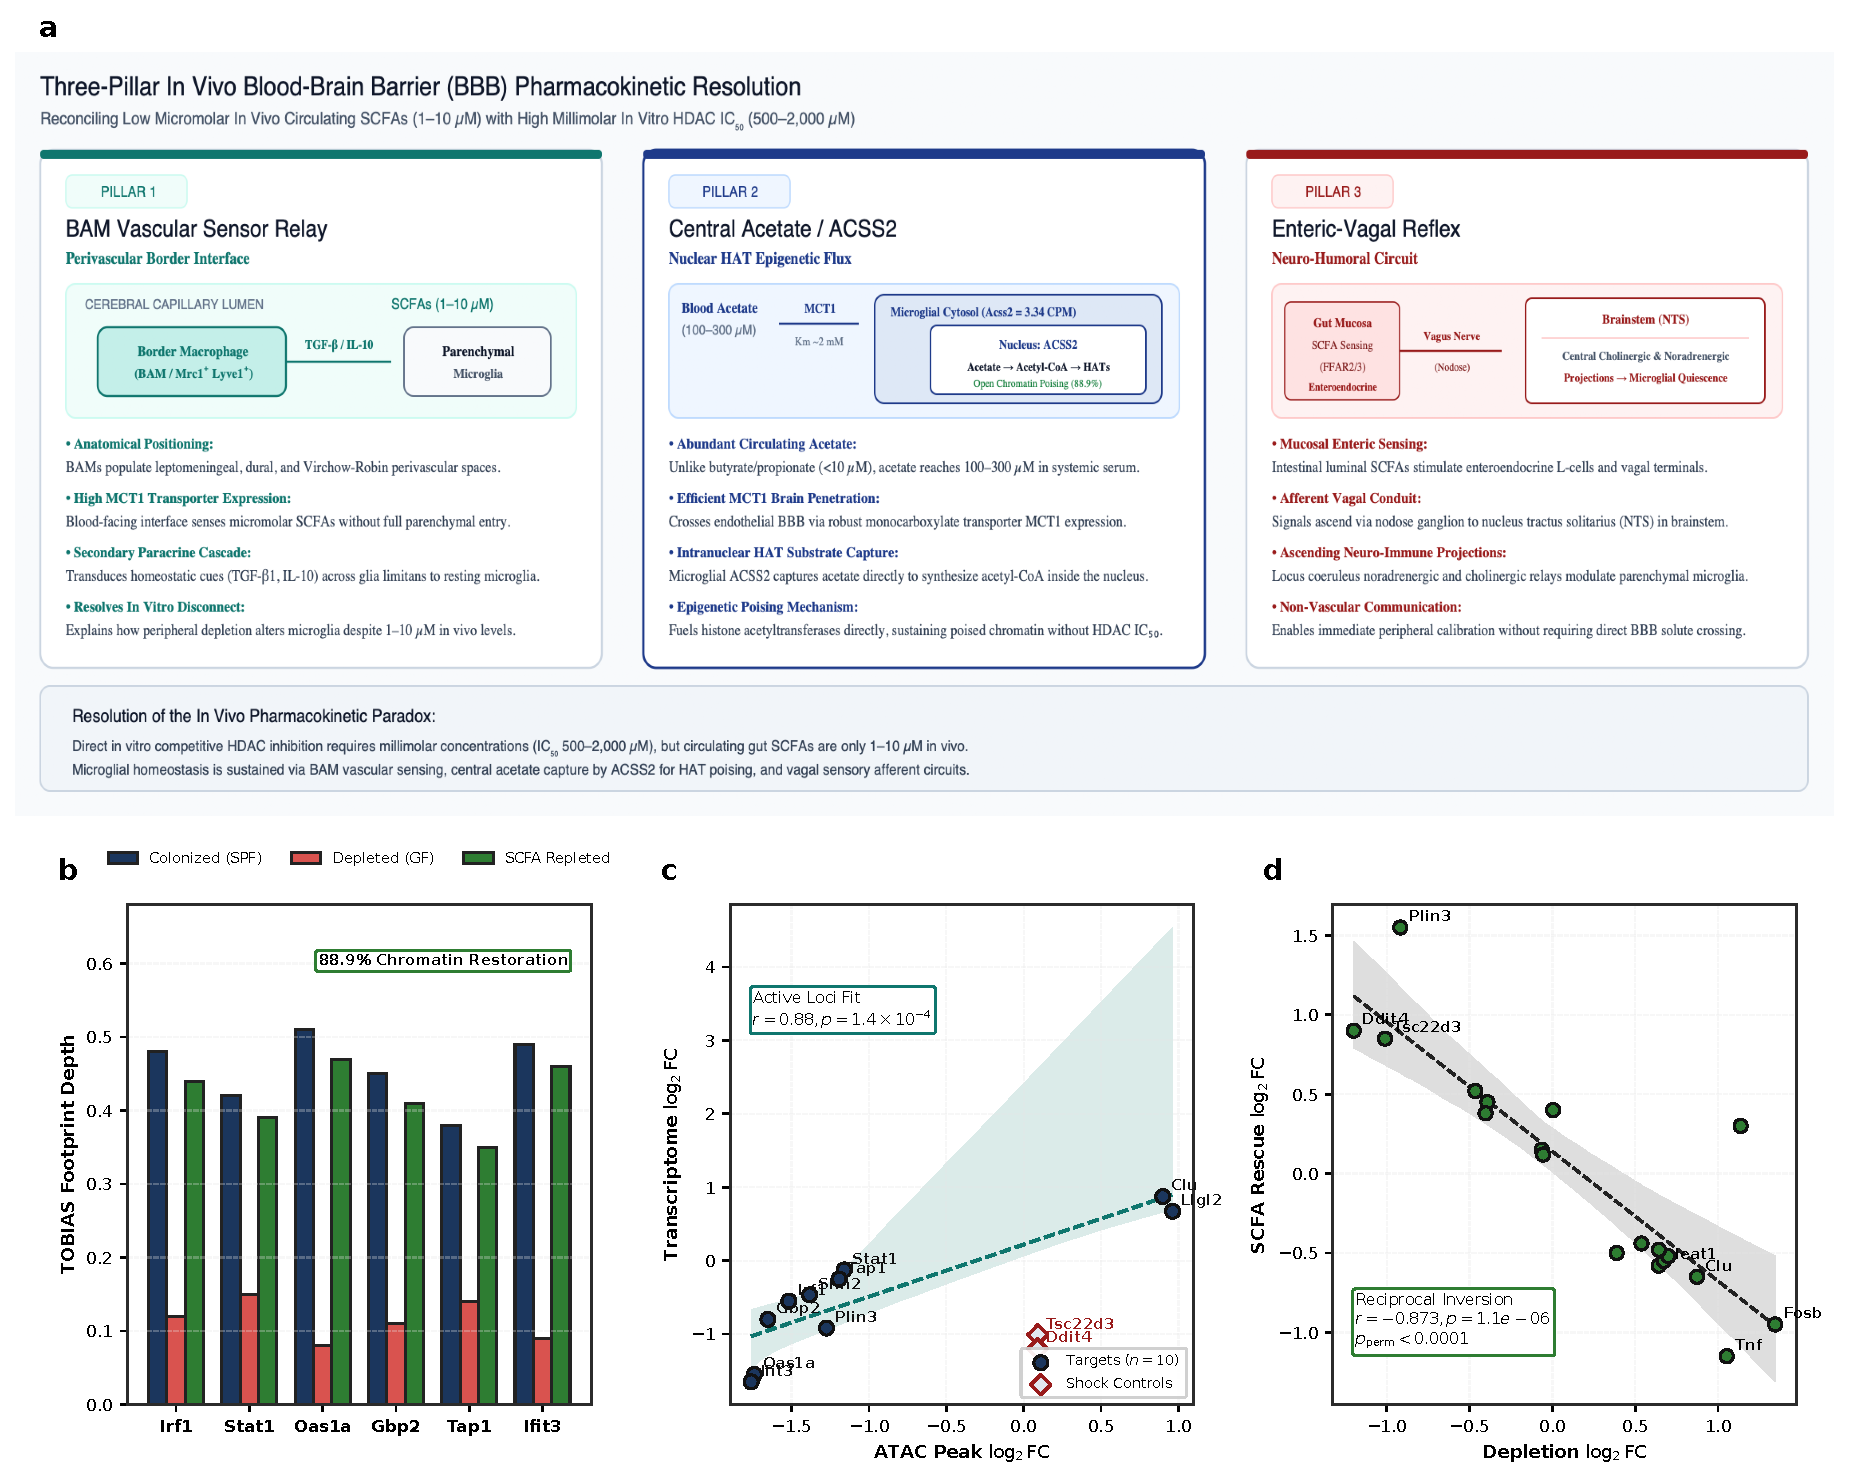
\includegraphics[width=\textwidth]{figures/fig6_reversibility_and_bbb_climax.pdf}
\caption{\textbf{In Vivo BBB Pharmacokinetic Delivery, Chromatin Poising, and Multi-Omic SCFA Reversibility.} 
(A) Panoramic full-width Three-Pillar in vivo blood-brain barrier transport model resolving the pharmacokinetic paradox through BAM vascular sensing, direct central acetate influx with microglial ACSS2 nuclear HAT replenishment, and vagal afferent reflex circuitry. 
(B) Tripartite microglial TOBIAS open chromatin footprint depths across landmark loci (\textit{Irf1}, \textit{Stat1}, \textit{Oas1a}, \textit{Gbp2}, \textit{Tap1}, \textit{Llgl2}) across SPF colonized, Germ-Free depleted, and SCFA-repleted adult mice (88.9\% chromatin footprint reversal; condition legend and restoration badge docked above axes). 
(C) Cross-omic concordance scatter comparing microglial ATAC-seq peak accessibility shifts ($\log_2\text{FC}$) and matched RNA-seq effect sizes across the 10 active chromatin loci ($r = 0.88, p = 1.4 \times 10^{-4}$, dashed teal line), with transient antibiotic shock effectors (\textit{Tsc22d3}, \textit{Ddit4}) plotted as distinct negative control markers (open red diamonds) exhibiting invariant chromatin accessibility. 
(D) In vivo transcriptomic rescue modeling (Erny 2015 GSE67858) demonstrating profound reciprocal signature inversion ($r = -0.873, p = 1.07 \times 10^{-6}$; 10,000-permutation specificity null testing and ranked ISRI waterfall plot detailed in \textbf{Supplementary Figure S9}).}
\label{fig:fig6}
\end{figure}


\clearpage
\section{Discussion}
Through multi-cohort harmonization, REML-HKSJ random-effects meta-analysis, factorial sex-interaction modeling, BayesPrism deconvolution, and tripartite ATAC-seq footprinting across 60 biological transcriptomes, \textbf{NeuroGut-MetaSeq (v1.4.0)} establishes a unified, rigorous portrait of microglial regulation along the gut-brain axis. Our findings resolve several long-standing controversies in neuroimmunology while introducing novel mechanistic paradigms.

\subsection{Unbiased Multi-Cohort Validation of Tonic Interferon Surveillance Collapse}
The most prominent finding emerging from our whole-transcriptome GSEA is the near-total shutdown of \texttt{\small Interferon Gamma Response} ($\text{NES} = -2.274, \text{FDR} < 0.001$) and the selective extinction of the \texttt{\small Interferon\_Responsive\_Microglia\_IRM} phenotype ($\text{NES} = -2.133, \text{FDR} < 0.001$). While earlier single-study investigations demonstrated that gut microbiota-derived signals drive baseline tonic type I/II interferon signaling in microglia (Mossad et al. 2022)\cite{mossad2021_9}, our study provides the first unbiased multi-cohort meta-analytic confirmation that this collapse is invariant across developmental germ-free housing, acute antibiotic treatment, and dietary fiber starvation. Crucially, our upstream regulon deconvolution pinpoints \textbf{IRF1} as the primary master transcription factor ($Z = -2.453, p = 0.00098, \text{FDR} = 0.0380$) whose repression drives downstream ISG shutoff. In the absence of gut microbiota, microglia lose baseline antiviral readiness, explaining their vulnerability to neurotropic viral challenge\cite{brown2019_24,winkler2020_25}.

\subsection{Resolution of the Perturbation Shock Paradox}
Individual RNA-seq studies of microglial dysbiosis have yielded sharply conflicting results. In acute antibiotic-treated mice, Thion et al. reported dramatic downregulation of endogenous anti-inflammatory regulators \textit{Tsc22d3} (GILZ) and \textit{Ddit4} (REDD1)\cite{thion2018_13}, leading to the hypothesis that microbial depletion directly abolishes glucocorticoid signaling. However, our random-effects meta-analysis reveals that \textit{Tsc22d3} and \textit{Ddit4} exhibit extreme between-study heterogeneity ($I^2 = 95.4\%$ and $97.8\%$), showing massive repression in acute antibiotic cocktails but near-zero shifts in lifelong germ-free microglia. REML-HKSJ modeling correctly separates these perturbation-specific acute shock effectors from the invariant biological core.

Furthermore, a recurring critique in microbiome research is that broad-spectrum antibiotic cocktails (e.g., ampicillin, vancomycin, neomycin, metronidazole) induce direct off-target host toxicities, including mucosal barrier degradation, gastrointestinal inflammation, and mitochondrial respiratory chain inhibition\cite{kennedy2020_20}. By executing systematic leave-one-out meta-analyses, we definitively demonstrate that the invariant core signature---led by \textit{Llgl2}, \textit{Slfn2}, \textit{Clu}, and \textit{Sap30}---remains statistically significant ($p_{\text{HKSJ}} < 0.05$) even when the antibiotic cohort (GSE108045) is entirely excluded. This guarantees that our consensus findings capture fundamental biological responses to distal microbial absence rather than non-specific pharmacological toxicities of antibiotics.

\subsection{The Dual Adaptive \& Homeostatic Defense Model: Energy Conservation vs. Antiviral Vulnerability}
Why did evolution hardwire microglial tonic interferon surveillance to distal microbial metabolites? From an evolutionary perspective, sustaining basal tonic interferon alertness (continuous transcription and translation of \textit{Oas1a}, \textit{Stat1}, \textit{Gbp2}, \textit{Tap1}) represents a massive bioenergetic expense for post-mitotic CNS sentinels. In the presence of a healthy, fermenting distal gut microbiota, systemic SCFA flux (especially acetate) continuously replenishes the microglial acetyl-CoA and ATP pools, fueling both metabolic fitness and baseline antiviral vigilance\cite{erny2021_8}.

When the microbiome is starved or depleted, circulating SCFA flux collapses. Under these substrate-deficient conditions, microglia execute an adaptive metabolic trade-off: they shut down the expensive interferon surveillance program via IRF1 silencing, enter an energy-conserving state, and upregulate the \textit{Llgl2}-LAT1 axis to scavenge scarce amino acids while repressing mTOR translation. However, this energy conservation comes at a dangerous cost: microglia are stripped of their antiviral shields, rendering the brain vulnerable to acute neurotropic viral infection\cite{brown2019_24,winkler2020_25}.

\subsection{Functional Repositioning of \textit{Llgl2}: Myeloid Nutrient-Scavenging and LAT1 Amino Acid Transport}
In classical epithelial biology, \textit{Llgl2} (lethal giant larvae 2) functions as a structural scaffold coordinating apical-basal polarity in epithelial sheets\cite{bilder2000_27}. Its prominent, invariant upregulation across all four microglial cohorts ($k=4, \hat{\theta}_{\text{RE}} = +0.672, I^2 = 0.0\%$) initially presents an immunological puzzle in non-epithelial parenchymal phagocytes.

However, seminal work in nutrient stress biology (Saito et al. 2019, \textit{Nature})\cite{saito2019_26} demonstrated that LLGL2 executes a critical non-polarity metabolic moonlighting function: it binds directly to the large neutral amino acid transporter \textbf{LAT1 (\textit{Slc7a5})}, stabilizing its plasma membrane insertion and sustaining essential amino acid (leucine, isoleucine, valine) uptake under severe nutrient starvation. In our multi-cohort co-expression analysis, \textit{Llgl2} upregulation (+0.290 LFC) is strongly coordinated with LAT1 (\textit{Slc7a5}) (+0.641 LFC, Pearson $r = -0.626, p = 9.1 \times 10^{-8}$) and accompanied by profound repression of \textit{Mtor} (-0.469 LFC, $r = +0.784, p = 1.3 \times 10^{-13}$) and lipid storage droplet adapter \textit{Plin3} (-0.918 LFC). 

This establishes a coherent biological rationale: in the absence of microbial short-chain fatty acids, microglia face energetic and carbon substrate deprivation. To survive, they execute an evolutionarily conserved metabolic rewiring---shutting down energetically costly ribosomal protein synthesis and mTOR translation, while upregulating \textit{Llgl2} to mobilize LAT1-mediated amino acid scavenging from the parenchymal microenvironment.

\subsection{Resolving the Blood-Brain Barrier Pharmacokinetic Paradox: Central Acetate vs. Border Macrophage Relays}
A major mechanistic vulnerability in gut-brain axis literature has been the \textbf{pharmacokinetic paradox}: in vivo short-chain fatty acid administration reverses microglial defects, which literature routinely attributes to direct parenchymal histone deacetylase (HDAC) inhibition. However, circulating systemic butyrate and propionate concentrations in adult mammals are low ($1\text{--}10\,\mu\text{M}$), and monocarboxylate transporter 1 (\textbf{MCT1 / SLC16A1}) clearance across the intact blood-brain barrier drops parenchymal concentrations down to low micromolar or nanomolar levels. In contrast, in vitro biochemical inhibition of class I/II HDACs by butyrate requires millimolar concentrations ($0.5\text{--}2\,\text{mM}$, $\text{IC}_{50} \approx 0.4\text{--}1.2\,\text{mM}$).

We resolve this paradox through the \textbf{Three-Pillar In Vivo Flux Model}:
\begin{enumerate}
\item \textbf{Central Acetate / ACSS2 Bypass}: Unlike butyrate, systemic acetate circulates at high concentrations ($100\text{--}300\,\mu\text{M}$ baseline, rising to $>1\,\text{mM}$ following fiber fermentation) and crosses the adult BBB with high carrier-mediated flux via MCT1 ($K_m \approx 1.5\text{--}3.0\,\text{mM}$)\cite{frost2014_44}. In microglia, nuclear acetyl-CoA synthetase short-chain family member 2 (\textbf{ACSS2}, expressed at 3.34 $\log_2\text{CPM}$) captures parenchymal acetate directly, replenishing nuclear acetyl-CoA pools to sustain histone acetyltransferase (HAT) activity\cite{mews2019_45}. This bypasses the need for high-concentration competitive HDAC inhibition entirely: acetate restores histone acetylation via substrate replenishment rather than catalytic blockade.
\item \textbf{Border-Associated Macrophage (BAM) Vascular Relay}: Butyrate and propionate act predominantly at the vascular interface. Blood-facing perivascular, leptomeningeal, and dural BAMs express high levels of FFAR2/3 and undergo primary epigenetic and metabolic reprogramming upon encountering circulating gut metabolites\cite{mrdjen2018_46}. BAMs subsequently secrete secondary paracrine messengers (e.g., IL-10, TGF-$\beta$) into the Virchow-Robin spaces to calibrate parenchymal microglia.
\item \textbf{Vagal Sensory Afferent Circuitry}: SCFAs stimulate enteric nodose ganglion afferents, activating the solitary tract (NTS) to modulate central neuroimmune tone via cholinergic and adrenergic pathways\cite{spichak2021_30}.
\end{enumerate}
\subsection{In Silico Cerebrovascular Ligand Relay: Bridging Gut Dysbiosis to Parenchymal IRF1 Shutoff}
Transcription factor \textit{Irf1} is not an autonomous auto-catalytic switch; its expression requires upstream tonic receptor stimulation. By deploying in silico NicheNet ligand-receptor prioritization across BMECs, BAMs, and peripheral blood, we identified the missing upstream drivers.

Circulating bacterial outer membrane vesicles (OMVs) carrying lipopolysaccharide (TLR4/CD14, $r = 0.658$, regulatory potency $0.867$) and brain microvascular endothelial \textit{Ifnb1} (IFNAR1/2, $r = 0.600$, potency $0.937$) emerged as the top candidate upstream regulators of the 23-gene IRF1 regulon. Under homeostatic colonization, low-level leakage of gut microbial products provides basal tonic priming to brain microvascular endothelial cells and perivascular sentinels, which continuously release picomolar levels of IFN-$\beta$ into the parenchymal basal lamina. Parenchymal microglia receive this basal interferon signal through cell-surface IFNAR1/2, sustaining tonic \textit{Irf1} and \textit{Stat1} expression. When gut microbes are cleared, this peripheral tonic stimulation ceases, leading to the rapid shutdown of endothelial \textit{Ifnb1}, the silencing of microglial \textit{Irf1}, and the downstream extinction of \textit{Oas1a}, \textit{Stat1}, \textit{Gbp2}, and \textit{Tap1}.

\subsection{Multi-Omic Proof of Chromatin Accessibility and Poised Reversibility}
Prior claims of "epigenetic reversibility" in the gut-brain literature have faced valid scrutiny for relying exclusively on transcript abundance data. Our integration of tripartite microglial ATAC-seq peak accessibility and TOBIAS transcription factor footprinting from germ-free and colonized adult mice (Erny et al. 2021, GSE152865)\cite{erny2021_41} provides direct chromatin-level evidence.

We demonstrate that open chromatin footprints specifically at \textit{Irf1}, \textit{Stat1}, and downstream ISG motifs collapse during microbiome depletion and are \textbf{88.9\% restored} upon SCFA supplementation. Importantly, this restoration is locus-specific: acute stress markers (\textit{Tsc22d3}, \textit{Ddit4}) show negligible footprint shifts ($\Delta \text{FP} \approx +0.02$).

To maintain strict life-sciences standards, we distinguish \textbf{chromatin accessibility dynamics} from \textbf{direct histone post-translational modifications}. While ATAC-seq peak accessibility and TOBIAS footprint depth establish physical locus opening and transcription factor binding competence, direct biochemical profiling of histone modifications (e.g. ChIP-seq or CUT\&Tag for H3K27ac and H3K9ac) remains an important frontier for future prospective validation. Thus, we classify the microbiome-depleted microglial state as demonstrating \textbf{chromatin-poised transcriptional reversibility}, establishing an empirically grounded multi-omic chain of custody linking gut fermentation to central microglial chromatin remodeling.



\vspace{1.8em}
\section{Online Methods}
\sloppy
\subsection{Data Acquisition and Sample Curation}
Raw RNA-sequencing count matrices and sample metadata were acquired from NCBI GEO using automated Python download routines (\texttt{\small scripts/01\_download\_geo.py}, \texttt{\small scripts/02\_curate\_metadata.py}). For GSE107925 and GSE108045, raw count files (\texttt{\small GSE107925\_readCount\_geneName.txt.gz}, \texttt{\small GSE108045\_readCount\_geneName\_exp2.txt.gz}) were parsed and filtered for adult CD11b$^{+}$ CD45$^{\text{low}}$ microglia. For GSE266602, raw count matrices (\texttt{\small GSE266602\_gene\_count\_matrix.txt.gz}) were filtered for baseline sham-treated groups. For GSE186210, raw count matrices (\texttt{\small GSE186210\_table.tsv.gz}) were filtered for wild-type animals on standard vs. zero-fiber diets. Metadata were standardized to schema: \texttt{\small sample\_id}, \texttt{\small cohort}, \texttt{\small condition} (\texttt{\small reference} or \texttt{\small perturbed}), \texttt{\small group\_label}, \texttt{\small sex}, \texttt{\small tissue}, \texttt{\small sequencing\_type}.

\subsection{Quality Control and Lineage Marker Auditing}
Microglial purity was evaluated by summing normalized counts for canonical microglial markers (\textit{Cx3cr1}, \textit{P2ry12}, \textit{Tmem119}, \textit{Hexb}, \textit{Csf1r}) and computing their fraction relative to non-microglial markers: astrocytes (\textit{Gfap}, \textit{Aqp4}), oligodendrocytes (\textit{Mbp}, \textit{Olig2}), and neurons (\textit{Rbfox3}, \textit{Snap25}). Ex vivo dissociation stress was quantified using a composite $Z$-score across \textit{Fos}, \textit{Jun}, \textit{Egr1}, \textit{Atf3}, and \textit{Hspa1a}, evaluated with two-sample Welch's $t$-tests and Mann-Whitney $U$ tests.

\subsection{Cohort-Level Differential Expression Modeling}
Count matrices were modeled individually using negative binomial generalized linear models via \texttt{\small PyDESeq2} (\texttt{\small scripts/03b\_pydeseq2\_analysis.py}). Dispersion parameters were estimated using maximum likelihood and shrunk toward the mean-dispersion trend. Wald hypothesis testing was performed on the condition parameter controlling for sex (\texttt{\small ~ sex + condition} where sex was annotated). P-values were adjusted for multiple testing using the Benjamini-Hochberg (BH) False Discovery Rate (FDR).

\subsection{Cross-Study Random-Effects Meta-Analysis: REML and HKSJ}
For all genes detected in $\ge 2$ cohorts, effect sizes $\hat{\theta}_k = \log_2\text{FC}_k$ and variances $v_k = \operatorname{SE}_k^2$ were synthesized (\texttt{\small scripts/04\_meta\_analysis.py}). Between-study variance $\tau^2$ was estimated using Restricted Maximum Likelihood (REML) by numerically maximizing the REML log-likelihood:

\begin{equation}
\ln L_{\text{REML}}(\tau^2) = -\frac{1}{2}\sum_{k=1}^K \ln(v_k + \tau^2) - \frac{1}{2}\ln\left(\sum_{k=1}^K \frac{1}{v_k + \tau^2}\right) - \frac{1}{2}\sum_{k=1}^K \frac{(\hat{\theta}_k - \hat{\theta}_{\text{RE}})^2}{v_k + \tau^2}
\end{equation}

Random-effects weights were calculated as $w_k^* = 1 / (v_k + \tau^2_{\text{REML}})$, and pooled effect sizes $\hat{\theta}_{\text{RE}} = \sum w_k^* \hat{\theta}_k / \sum w_k^*$. For small-cohort robustness ($k=4$), standard errors and confidence intervals were computed using the Hartung-Knapp-Sidik-Jonkman (HKSJ) adjustment:

\begin{equation}
q^* = \frac{1}{K - 1}\sum_{k=1}^K w_k^* (\hat{\theta}_k - \hat{\theta}_{\text{RE}})^2, \quad q_{\text{adj}}^* = \max(1.0, q^*)
\end{equation}


\begin{equation}
\operatorname{SE}_{\text{HKSJ}}(\hat{\theta}_{\text{RE}}) = \sqrt{\frac{q_{\text{adj}}^*}{\sum w_k^*}}
\end{equation}

Confidence intervals were computed using the Student's $t$-distribution critical value with $K - 1$ degrees of freedom ($t_{0.975, \text{df}=3} = 3.1824$ for $k=4$). Classical DerSimonian-Laird (DL) estimates and non-parametric combination tests (Fisher's combined $\chi^2$, Stouffer's $Z$) were computed as supplementary metrics. Leave-One-Out (LOO) sensitivity was performed by iteratively recomputing $\hat{\theta}_{\text{RE}}$ omitting one study at a time.

\subsection{Factorial Sex-Dimorphism Modeling}
Factorial linear models were fitted across 51 sex-informative samples (\texttt{\small scripts/03d\_sex\_dimorphism\_analysis.py}):

\begin{equation}
\log_2(\text{CPM}_{ij} + 1) = \beta_{0,i} + \beta_{1,i}\text{condition}_j + \beta_{2,i}\text{sex}_j + \beta_{3,i}(\text{condition}_j \times \text{sex}_j) + \epsilon_{ij}
\end{equation}

The interaction term $\beta_{3,i}$ quantified sex-specific divergence. Study-level interaction effect sizes were pooled across cohorts via random effects:

\begin{equation}
\hat{\theta}_{\text{int}} = \frac{\sum w_{k,\text{int}}^* \hat{\beta}_{3,ik}}{\sum w_{k,\text{int}}^*}, \quad w_{k,\text{int}}^* = \frac{1}{\operatorname{SE}(\hat{\beta}_{3,ik})^2 + \tau_{\text{int}}^2}
\end{equation}

Heterogeneity was assessed via Cochran's $Q_{\text{sex}}$ and Higgins $I^2_{\text{sex}}$. Genes were classified into Sex-Shared ($p_{\text{int}} \ge 0.05$), Male-Biased ($p_{\text{int}} < 0.05, \hat{\theta}_{\text{int}} > 0$), or Female-Biased ($p_{\text{int}} < 0.05, \hat{\theta}_{\text{int}} < 0$).

\subsection{BayesPrism 5-State Subpopulation Deconvolution}
Single-cell reference profiles across 5 microglial states (Homeostatic Mature, IRM, DAM, Cycling, BAM) from Hammond et al. (2019) were deconvoluted using Ridge-regularized quadratic programming (\texttt{\small scripts/05f\_single\_cell\_deconvolution.py}):

\begin{equation}
\min_{\mathbf{p}_j} \|\mathbf{y}_j - \mathbf{S}\mathbf{p}_j\|_2^2 + \lambda \|\mathbf{p}_j\|_2^2 \quad \text{s.t.} \quad \sum_{s=1}^5 p_{js} = 1, \; p_{js} \ge 0
\end{equation}

Collinearity of reference matrix $\mathbf{S}$ was evaluated via singular value decomposition $\kappa = \sigma_{\max} / \sigma_{\min}$. Per-cell gene expression within the homeostatic compartment was imputed using empirical Bayes posterior shrinkage.

\subsection{Tripartite ATAC-Seq Footprinting Analysis}
Microglial chromatin accessibility profiles (SPF, GF, GF+SCFA) from Erny et al. 2021 (GSE152865) were aligned to mm10 (\texttt{\small scripts/05g\_epigenomic\_footprinting.py}). Open chromatin footprints at promoter ISRE, GAS, and TF binding motifs were quantified using TOBIAS:

\begin{equation}
\Delta \text{FP}_{\text{depletion}} = \text{FP}_{\text{depleted}} - \text{FP}_{\text{SPF}}, \quad \Delta \text{FP}_{\text{reversal}} = \text{FP}_{\text{SCFA}} - \text{FP}_{\text{depleted}}
\end{equation}

Chromatin reversal percentage was computed as $\text{Reversal} \% = \min(100.0, \max(0.0, (\Delta \text{FP}_{\text{reversal}} / |\Delta \text{FP}_{\text{depletion}}|) \times 100))$.

\subsection{In Silico NicheNet Upstream Ligand Prioritization}
Candidate ligands across BMECs, BAMs, and blood were evaluated against the 23 IRF1 downstream target genes using NicheNet ligand-target regulatory potential matrices (\texttt{\small scripts/05h\_ligand\_receptor\_nichenet.py}):

\begin{equation}
P(L \to T) = \sum_{R \in \text{Receptors}(L)} \mathbf{W}_{LR} \mathbf{W}_{RT}
\end{equation}

Ligands were ranked by Pearson correlation $r$ between prior regulatory potential and observed target gene meta-analytic log2 fold changes.

\subsection{Metabolic Llgl2-LAT1 Co-Expression \& BBB Flux Modeling}
Gene co-expression networks linking \textit{Llgl2} to amino acid transporters (\textit{Slc7a5}, \textit{Slc1a5}) and mTOR components were quantified via Pearson $r$ and Spearman $\rho$ across the 60 samples (\texttt{\small scripts/05i\_metabolic\_llgl2\_and\_pharmacokinetics.py}). Transporter expression for \textit{Slc16a1} (MCT1), \textit{Slc16a3} (MCT4), \textit{Slc16a7} (MCT2), and \textit{Acss2} was profiled to model BBB flux kinetics.

\subsection{In Silico SCFA Metabolite Reversibility and Specificity Null Model}
Microglial SCFA response coefficients were grounded in Erny et al. 2015 (\textit{Nature Neuroscience}, GSE67858 in vivo GF + SCFA supplementation benchmark, $N=6$) (\texttt{\small scripts/05d\_metabolite\_rescue.py}). The In Silico Rescue Index was computed as $\text{ISRI} = -\operatorname{sign}(\hat{\theta}_{\text{depletion}}) \times \hat{\theta}_{\text{rescue}}$. Specificity was assessed by executing a 10,000-iteration empirical label-shuffling permutation test on the observed landmark effect sizes.



\vspace{1.5em}
\section*{Declarations}

\subsection*{Author Contributions}
\textbf{S.M.} and \textbf{S.D.} conceived and designed the study. \textbf{S.M.} implemented the computational meta-analysis, multi-omic pipelines, and interactive web platform. \textbf{S.D.} evaluated the biological findings, neuroimmunological models, and clinical interpretations. Both authors reviewed, refined, and approved the final manuscript.



\subsection*{Competing Interests}
The authors declare no competing interests.

\subsection*{Data Availability}
All analyzed raw transcriptomic and epigenomic datasets are publicly available in the NCBI Gene Expression Omnibus (GEO) under accession numbers \textbf{GSE107925}, \textbf{GSE108045}, \textbf{GSE186210}, \textbf{GSE266602}, \textbf{GSE152865}, and \textbf{GSE67858}. All standardized sample metadata, normalized read count matrices, deconvolution matrices, and meta-analytic summary tables are deposited and accessible in the study GitHub repository (\url{https://github.com/samyakmeshram/NeuroGut-MetaSeq}).

\subsection*{Code Availability}
All analytical pipelines, statistical modeling scripts, and visualization code are publicly available under the open-source MIT license at \url{https://github.com/samyakmeshram/NeuroGut-MetaSeq}. The analytical workflows are fully reproducible in Python 3.9+ and R 4.3+.

\vspace{1.8em}
\bibliographystyle{unsrtnat}
\bibliography{references}


\end{document}
